% ****************************************************************************************
% *****************          PRACTICA 3: SENSOR INFRARROJO     ***************************
% ****************************************************************************************


% =======================================================
% =======         HEADER FOR DOCUMENT        ============
% =======================================================
    
    % *********   HEADERS AND FOOTERS ********
    \def\ProjectAuthorLink{https://github.com/SoyOscarRH}           %Just to keep it in line
    \def\ProjectNameLink{https://github.com/CompilandoConocimiento} %Just to keep it in line

    % *********   DOCUMENT ITSELF   **************
    \documentclass[12pt, fleqn]{article}                            %Type of docuemtn and size of font and left eq
    \usepackage[margin = 1.2in]{geometry}                           %Margins and Geometry pacakge
    \usepackage[spanish]{babel}                                     %Please use spanish
    \usepackage[utf8]{inputenc}                                     %Please use spanish - UFT
    \usepackage{ifthen}                                             %Allow simple programming
    \usepackage{hyperref}                                           %Create MetaData for a PDF and LINKS!
    \usepackage{pdfpages}                                           %Create MetaData for a PDF and LINKS!
    \hypersetup{pageanchor = false}                                 %Solve 'double page 1' warnings in build
    \setlength{\parindent}{0pt}                                     %Eliminate ugly indentation
    \author{Oscar Andrés Rosas}                                     %Who I am

    % *********   LANGUAJE AND UFT-8   *********
    \usepackage[T1]{fontenc}                                        %Please use spanish
    \usepackage{textcmds}                                           %Allow us to use quoutes
    \usepackage{changepage}                                         %Allow us to use identate paragraphs
    \usepackage{anyfontsize}                                        %All the sizes

    % *********   MATH AND HIS STYLE  *********
    \usepackage{ntheorem, amsmath, amssymb, amsfonts}               %All fucking math, I want all!
    \usepackage{mathrsfs, mathtools, empheq}                        %All fucking math, I want all!
    \usepackage{cancel}                                             %Negate symbol
    \usepackage{centernot}                                          %Allow me to negate a symbol
    \decimalpoint                                                   %Use decimal point

    % *********   GRAPHICS AND IMAGES *********
    \usepackage{graphicx}                                           %Allow to create graphics
    \usepackage{float}                                              %For images
    \usepackage{wrapfig}                                            %Allow to create images
    \graphicspath{ {Graphics/} }                                    %Where are the images :D

    % *********   LISTS AND TABLES ***********
    \usepackage{listings, listingsutf8}                             %We will be using code here
    \usepackage[inline]{enumitem}                                   %We will need to enumarate
    \usepackage{tasks}                                              %Horizontal lists
    \usepackage{longtable}                                          %Lets make tables awesome
    \usepackage{booktabs}                                           %Lets make tables awesome
    \usepackage{tabularx}                                           %Lets make tables awesome
    \usepackage{multirow}                                           %Lets make tables awesome
    \usepackage{multicol}                                           %Create multicolumns

    % *********   HEADERS AND FOOTERS ********
    \usepackage{fancyhdr}                                           %Lets make awesome headers/footers
    \pagestyle{fancy}                                               %Lets make awesome headers/footers
    \setlength{\headheight}{16pt}                                   %Top line
    \setlength{\parskip}{0.5em}                                     %Top line
    \renewcommand{\footrulewidth}{0.5pt}                            %Bottom line

    \lhead{                                                         %Left Header
        \hyperlink{section.\arabic{section}}                        %Make a link to the current chapter
        {\normalsize{\textsc{\nouppercase{\leftmark}}}}             %And fot it put the name
    }

    \rhead{                                                         %Right Header
        \hyperlink{section.\arabic{section}.\arabic{subsection}}    %Make a link to the current chapter
            {\footnotesize{\textsc{\nouppercase{\rightmark}}}}      %And fot it put the name
    }

    \rfoot{\textsc{\small{\hyperref[sec:Index]{Ve al Índice}}}}     %This will always be a footer  

    \fancyfoot[L]{                                                  %Algoritm for a changing footer
        \ifthenelse{\isodd{\value{page}}}                           %IF ODD PAGE:
            {\href{https://compilandoconocimiento.com/nosotros/}    %DO THIS:
                {\footnotesize                                      %Send the page
                    {\textsc{Oscar Andrés Rosas}}}}                 %Send the page
            {\href{https://compilandoconocimiento.com}              %ELSE DO THIS: 
                {\footnotesize                                      %Send the author
                    {\textsc{Laura Andres Morales}}}}               %Send the author
    }
    
    
    
% =======================================================
% ===================   COMMANDS    =====================
% =======================================================

    % =========================================
    % =======   NEW ENVIRONMENTS   ============
    % =========================================
    \newenvironment{Indentation}[1][0.75em]                         %Use: \begin{Inde...}[Num]...\end{Inde...}
        {\begin{adjustwidth}{#1}{}}                                 %If you dont put nothing i will use 0.75 em
        {\end{adjustwidth}}                                         %This indentate a paragraph
    \newenvironment{SmallIndentation}[1][0.75em]                    %Use: The same that we upper one, just 
        {\begin{adjustwidth}{#1}{}\begin{footnotesize}}             %footnotesize size of letter by default
        {\end{footnotesize}\end{adjustwidth}}                       %that's it

    \newenvironment{MultiLineEquation}[1]                           %Use: To create MultiLine equations
        {\begin{equation}\begin{alignedat}{#1}}                     %Use: \begin{Multi..}{Num. de Columnas}
        {\end{alignedat}\end{equation}}                             %And.. that's it!
    \newenvironment{MultiLineEquation*}[1]                          %Use: To create MultiLine equations
        {\begin{equation*}\begin{alignedat}{#1}}                    %Use: \begin{Multi..}{Num. de Columnas}
        {\end{alignedat}\end{equation*}}                            %And.. that's it!
    

    % =========================================
    % == GENERAL TEXT & SYMBOLS ENVIRONMENTS ==
    % =========================================
    
    % =====  TEXT  ======================
    \newcommand \Quote {\qq}                                        %Use: \Quote to use quotes
    \newcommand \Over {\overline}                                   %Use: \Bar to use just for short
    \newcommand \ForceNewLine {$\Space$\\}                          %Use it in theorems for example

    % =====  SPACES  ====================
    \DeclareMathOperator \Space {\quad}                             %Use: \Space for a cool mega space
    \DeclareMathOperator \MegaSpace {\quad \quad}                   %Use: \MegaSpace for a cool mega mega space
    \DeclareMathOperator \MiniSpace {\;}                            %Use: \Space for a cool mini space
    
    % =====  MATH TEXT  =================
    \newcommand \Such {\MiniSpace | \MiniSpace}                     %Use: \Such like in sets
    \newcommand \Also {\MiniSpace \text{y} \MiniSpace}              %Use: \Also so it's look cool
    \newcommand \Remember[1]{\Space\text{\scriptsize{#1}}}          %Use: \Remember so it's look cool
    
    % =====  THEOREMS  ==================
    \newtheorem{Theorem}{Teorema}[section]                          %Use: \begin{Theorem}[Name]\label{Nombre}...
    \newtheorem{Corollary}{Colorario}[Theorem]                      %Use: \begin{Corollary}[Name]\label{Nombre}...
    \newtheorem{Lemma}[Theorem]{Lemma}                              %Use: \begin{Lemma}[Name]\label{Nombre}...
    \newtheorem{Definition}{Definición}[section]                    %Use: \begin{Definition}[Name]\label{Nombre}...
    \theoremstyle{break}                                            %THEOREMS START 1 SPACE AFTER

    % =====  LOGIC  =====================
    \newcommand \lIff {\leftrightarrow}                             %Use: \lIff for logic iff
    \newcommand \lEqual {\MiniSpace \Leftrightarrow \MiniSpace}     %Use: \lEqual for a logic double arrow
    \newcommand \lInfire {\MiniSpace \Rightarrow \MiniSpace}        %Use: \lInfire for a logic infire
    \newcommand \lLongTo {\longrightarrow}                          %Use: \lLongTo for a long arrow

    % =====  FAMOUS SETS  ===============
    \DeclareMathOperator \Naturals     {\mathbb{N}}                 %Use: \Naturals por Notation
    \DeclareMathOperator \Primes       {\mathbb{P}}                 %Use: \Primes por Notation
    \DeclareMathOperator \Integers     {\mathbb{Z}}                 %Use: \Integers por Notation
    \DeclareMathOperator \Racionals    {\mathbb{Q}}                 %Use: \Racionals por Notation
    \DeclareMathOperator \Reals        {\mathbb{R}}                 %Use: \Reals por Notation
    \DeclareMathOperator \Complexs     {\mathbb{C}}                 %Use: \Complex por Notation
    \DeclareMathOperator \GenericField {\mathbb{F}}                 %Use: \GenericField por Notation
    \DeclareMathOperator \VectorSet    {\mathbb{V}}                 %Use: \VectorSet por Notation
    \DeclareMathOperator \SubVectorSet {\mathbb{W}}                 %Use: \SubVectorSet por Notation
    \DeclareMathOperator \Polynomials  {\mathbb{P}}                 %Use: \Polynomials por Notation

    % =====  CONTAINERS   ===============
    \newcommand{\Set}[1]{\left\{ \; #1 \; \right\}}                 %Use: \Set {Info} for INTELLIGENT space 
    \newcommand{\bigSet}[1]{\big\{ \; #1 \; \big\}}                 %Use: \bigSet  {Info} for space 
    \newcommand{\BigSet}[1]{\Big\{ \; #1 \; \Big\}}                 %Use: \BigSet  {Info} for space 
    \newcommand{\biggSet}[1]{\bigg\{ \; #1 \; \bigg\}}              %Use: \biggSet {Info} for space 
    \newcommand{\BiggSet}[1]{\Bigg\{ \; #1 \; \Bigg\}}              %Use: \BiggSet {Info} for space 
    
    \newcommand{\Brackets}[1]{\left[ #1 \right]}                    %Use: \Brackets {Info} for INTELLIGENT space
    \newcommand{\bigBrackets}[1]{\big[ \; #1 \; \big]}              %Use: \bigBrackets  {Info} for space 
    \newcommand{\BigBrackets}[1]{\Big[ \; #1 \; \Big]}              %Use: \BigBrackets  {Info} for space 
    \newcommand{\biggBrackets}[1]{\bigg[ \; #1 \; \bigg]}           %Use: \biggBrackets {Info} for space 
    \newcommand{\BiggBrackets}[1]{\Bigg[ \; #1 \; \Bigg]}           %Use: \BiggBrackets {Info} for space 
    
    \newcommand{\Wrap}[1]{\left( #1 \right)}                        %Use: \Wrap {Info} for INTELLIGENT space
    \newcommand{\bigWrap}[1]{\big( \; #1 \; \big)}                  %Use: \bigBrackets  {Info} for space 
    \newcommand{\BigWrap}[1]{\Big( \; #1 \; \Big)}                  %Use: \BigBrackets  {Info} for space 
    \newcommand{\biggWrap}[1]{\bigg( \; #1 \; \bigg)}               %Use: \biggBrackets {Info} for space 
    \newcommand{\BiggWrap}[1]{\Bigg( \; #1 \; \Bigg)}               %Use: \BiggBrackets {Info} for space 

    % =====  BETTERS MATH COMMANDS   =====
    \newcommand{\pfrac}[2]{\Wrap{\dfrac{#1}{#2}}}                   %Use: Put fractions in parentesis

    % =========================================
    % ====   LINEAL ALGEBRA & VECTORS    ======
    % =========================================

    % ===== UNIT VECTORS  ================
    \newcommand{\hati} {\hat{\imath}}                               %Use: \hati for unit vector    
    \newcommand{\hatj} {\hat{\jmath}}                               %Use: \hatj for unit vector    
    \newcommand{\hatk} {\hat{k}}                                    %Use: \hatk for unit vector

    % ===== MAGNITUDE  ===================
    \newcommand{\abs}[1]{\left\lvert #1 \right\lvert}               %Use: \abs{expression} for |x|
    \newcommand{\Abs}[1]{\left\lVert #1 \right\lVert}               %Use: \Abs{expression} for ||x||
    \newcommand{\Mag}[1]{\left| #1 \right|}                         %Use: \Mag {Info} 
    
    \DeclareMathOperator \LinealTransformation {\mathcal{T}}        %Use: \LinealTransformation for a cool T
    \newcommand{\bVec}[1]{\mathbf{#1}}                              %Use for bold type of vector
    \newcommand{\lVec}[1]{\overrightarrow{#1}}                      %Use for a long arrow over a vector
    \newcommand{\uVec}[1]{\mathbf{\hat{#1}}}                        %Use: Unitary Vector Example: $\uVec{i}

    % ===== ALL FOR DOT PRODUCT  =========
    \makeatletter                                                   %WTF! IS THIS
    \newcommand*\dotP{\mathpalette\dotP@{.5}}                       %Use: \dotP for dot product
    \newcommand*\dotP@[2] {\mathbin {                               %WTF! IS THIS            
        \vcenter{\hbox{\scalebox{#2}{$\m@th#1\bullet$}}}}           %WTF! IS THIS
    }                                                               %WTF! IS THIS
    \makeatother                                                    %WTF! IS THIS

    % === WRAPPERS FOR COLUMN VECTOR ===
    \newcommand{\pVector}[1]                                        %Use: \pVector {Matrix Notation} use parentesis
        { \ensuremath{\begin{pmatrix}#1\end{pmatrix}} }             %Example: \pVector{a\\b\\c} or \pVector{a&b&c} 
    \newcommand{\lVector}[1]                                        %Use: \lVector {Matrix Notation} use a abs 
        { \ensuremath{\begin{vmatrix}#1\end{vmatrix}} }             %Example: \lVector{a\\b\\c} or \lVector{a&b&c} 
    \newcommand{\bVector}[1]                                        %Use: \bVector {Matrix Notation} use a brackets 
        { \ensuremath{\begin{bmatrix}#1\end{bmatrix}} }             %Example: \bVector{a\\b\\c} or \bVector{a&b&c} 
    \newcommand{\Vector}[1]                                         %Use: \Vector {Matrix Notation} no parentesis
        { \ensuremath{\begin{matrix}#1\end{matrix}} }               %Example: \Vector{a\\b\\c} or \Vector{a&b&c}

    % === MAKE MATRIX BETTER  =========
    \makeatletter                                                   %Example: \begin{matrix}[cc|c]
    \renewcommand*\env@matrix[1][*\c@MaxMatrixCols c] {             %WTF! IS THIS
        \hskip -\arraycolsep                                        %WTF! IS THIS
        \let\@ifnextchar\new@ifnextchar                             %WTF! IS THIS
        \array{#1}                                                  %WTF! IS THIS
    }                                                               %WTF! IS THIS
    \makeatother                                                    %WTF! IS THIS

    % =========================================
    % =======   FAMOUS FUNCTIONS   ============
    % =========================================

    % == TRIGONOMETRIC FUNCTIONS  ====
    \newcommand{\Cos}[1] {\cos\Wrap{#1}}                            %Simple wrappers
    \newcommand{\Sin}[1] {\sin\Wrap{#1}}                            %Simple wrappers
    \newcommand{\Tan}[1] {tan\Wrap{#1}}                             %Simple wrappers
    
    \newcommand{\Sec}[1] {sec\Wrap{#1}}                             %Simple wrappers
    \newcommand{\Csc}[1] {csc\Wrap{#1}}                             %Simple wrappers
    \newcommand{\Cot}[1] {cot\Wrap{#1}}                             %Simple wrappers

    % === COMPLEX ANALYSIS TRIG ======
    \newcommand \Cis[1]  {\Cos{#1} + i \Sin{#1}}                    %Use: \Cis for cos(x) + i sin(x)
    \newcommand \pCis[1] {\Wrap{\Cis{#1}}}                          %Use: \pCis for the same with parantesis
    \newcommand \bCis[1] {\Brackets{\Cis{#1}}}                      %Use: \bCis for the same with Brackets


    % =========================================
    % ===========     CALCULUS     ============
    % =========================================

    % ====== TRANSFORMS =============
    \newcommand{\FourierT}[1]{\mathscr{F} \left\{ #1 \right\} }     %Use: \FourierT {Funtion}
    \newcommand{\InvFourierT}[1]{\mathscr{F}^{-1}\left\{#1\right\}} %Use: \InvFourierT {Funtion}

    % ====== DERIVATIVES ============
    \newcommand \MiniDerivate[1][x] {\dfrac{d}{d #1}}               %Use: \MiniDerivate[var] for simple use [var]
    \newcommand \Derivate[2] {\dfrac{d \; #1}{d #2}}                %Use: \Derivate [f(x)][x]
    \newcommand \MiniUpperDerivate[2] {\dfrac{d^{#2}}{d#1^{#2}}}    %Mini Derivate High Orden Derivate -- [x][pow]
    \newcommand \UpperDerivate[3] {\dfrac{d^{#3} \; #1}{d#2^{#3}}}  %Complete High Orden Derivate -- [f(x)][x][pow]
    
    \newcommand \MiniPartial[1][x] {\dfrac{\partial}{\partial #1}}  %Use: \MiniDerivate for simple use [var]
    \newcommand \Partial[2] {\dfrac{\partial \; #1}{\partial #2}}   %Complete Partial Derivate -- [f(x)][x]
    \newcommand \MiniUpperPartial[2]                                %Mini Derivate High Orden Derivate -- [x][pow] 
        {\dfrac{\partial^{#2}}{\partial #1^{#2}}}                   %Mini Derivate High Orden Derivate
    \newcommand \UpperPartial[3]                                    %Complete High Orden Derivate -- [f(x)][x][pow]
        {\dfrac{\partial^{#3} \; #1}{\partial#2^{#3}}}              %Use: \UpperDerivate for simple use

    \DeclareMathOperator \Evaluate  {\Big|}                         %Use: \Evaluate por Notation

    % =========================================
    % ========    GENERAL STYLE     ===========
    % =========================================
    
    % =====  COLORS ==================
    \definecolor{RedMD}{HTML}{F44336}                               %Use: Color :D        
    \definecolor{Red100MD}{HTML}{FFCDD2}                            %Use: Color :D        
    \definecolor{Red200MD}{HTML}{EF9A9A}                            %Use: Color :D        
    \definecolor{Red300MD}{HTML}{E57373}                            %Use: Color :D        
    \definecolor{Red700MD}{HTML}{D32F2F}                            %Use: Color :D 

    \definecolor{PurpleMD}{HTML}{9C27B0}                            %Use: Color :D        
    \definecolor{Purple100MD}{HTML}{E1BEE7}                         %Use: Color :D        
    \definecolor{Purple200MD}{HTML}{EF9A9A}                         %Use: Color :D        
    \definecolor{Purple300MD}{HTML}{BA68C8}                         %Use: Color :D        
    \definecolor{Purple700MD}{HTML}{7B1FA2}                         %Use: Color :D 

    \definecolor{IndigoMD}{HTML}{3F51B5}                            %Use: Color :D        
    \definecolor{Indigo100MD}{HTML}{C5CAE9}                         %Use: Color :D        
    \definecolor{Indigo200MD}{HTML}{9FA8DA}                         %Use: Color :D        
    \definecolor{Indigo300MD}{HTML}{7986CB}                         %Use: Color :D        
    \definecolor{Indigo700MD}{HTML}{303F9F}                         %Use: Color :D 

    \definecolor{BlueMD}{HTML}{2196F3}                              %Use: Color :D        
    \definecolor{Blue100MD}{HTML}{BBDEFB}                           %Use: Color :D        
    \definecolor{Blue200MD}{HTML}{90CAF9}                           %Use: Color :D        
    \definecolor{Blue300MD}{HTML}{64B5F6}                           %Use: Color :D        
    \definecolor{Blue700MD}{HTML}{1976D2}                           %Use: Color :D        
    \definecolor{Blue900MD}{HTML}{0D47A1}                           %Use: Color :D  

    \definecolor{CyanMD}{HTML}{00BCD4}                              %Use: Color :D        
    \definecolor{Cyan100MD}{HTML}{B2EBF2}                           %Use: Color :D        
    \definecolor{Cyan200MD}{HTML}{80DEEA}                           %Use: Color :D        
    \definecolor{Cyan300MD}{HTML}{4DD0E1}                           %Use: Color :D        
    \definecolor{Cyan700MD}{HTML}{0097A7}                           %Use: Color :D        
    \definecolor{Cyan900MD}{HTML}{006064}                           %Use: Color :D 

    \definecolor{TealMD}{HTML}{009688}                              %Use: Color :D        
    \definecolor{Teal100MD}{HTML}{B2DFDB}                           %Use: Color :D        
    \definecolor{Teal200MD}{HTML}{80CBC4}                           %Use: Color :D        
    \definecolor{Teal300MD}{HTML}{4DB6AC}                           %Use: Color :D        
    \definecolor{Teal700MD}{HTML}{00796B}                           %Use: Color :D        
    \definecolor{Teal900MD}{HTML}{004D40}                           %Use: Color :D 

    \definecolor{GreenMD}{HTML}{4CAF50}                             %Use: Color :D        
    \definecolor{Green100MD}{HTML}{C8E6C9}                          %Use: Color :D        
    \definecolor{Green200MD}{HTML}{A5D6A7}                          %Use: Color :D        
    \definecolor{Green300MD}{HTML}{81C784}                          %Use: Color :D        
    \definecolor{Green700MD}{HTML}{388E3C}                          %Use: Color :D        
    \definecolor{Green900MD}{HTML}{1B5E20}                          %Use: Color :D

    \definecolor{AmberMD}{HTML}{FFC107}                             %Use: Color :D        
    \definecolor{Amber100MD}{HTML}{FFECB3}                          %Use: Color :D        
    \definecolor{Amber200MD}{HTML}{FFE082}                          %Use: Color :D        
    \definecolor{Amber300MD}{HTML}{FFD54F}                          %Use: Color :D        
    \definecolor{Amber700MD}{HTML}{FFA000}                          %Use: Color :D        
    \definecolor{Amber900MD}{HTML}{FF6F00}                          %Use: Color :D

    \definecolor{BlueGreyMD}{HTML}{607D8B}                          %Use: Color :D        
    \definecolor{BlueGrey100MD}{HTML}{CFD8DC}                       %Use: Color :D        
    \definecolor{BlueGrey200MD}{HTML}{B0BEC5}                       %Use: Color :D        
    \definecolor{BlueGrey300MD}{HTML}{90A4AE}                       %Use: Color :D        
    \definecolor{BlueGrey700MD}{HTML}{455A64}                       %Use: Color :D        
    \definecolor{BlueGrey900MD}{HTML}{263238}                       %Use: Color :D        

    \definecolor{DeepPurpleMD}{HTML}{673AB7}                        %Use: Color :D

    \newcommand{\Color}[2]{\textcolor{#1}{#2}}                      %Simple color environment
    \newenvironment{ColorText}[1]                                   %Use: \begin{ColorText}
        { \leavevmode\color{#1}\ignorespaces }                      %That's is!

    % =====  CODE EDITOR =============
    \lstdefinestyle{CompilandoStyle} {                              %This is Code Style
        backgroundcolor     = \color{BlueGrey900MD},                %Background Color  
        basicstyle          = \tiny\color{white},                   %Style of text
        commentstyle        = \color{BlueGrey200MD},                %Comment style
        stringstyle         = \color{Green300MD},                   %String style
        keywordstyle        = \color{Blue300MD},                    %keywords style
        numberstyle         = \tiny\color{TealMD},                  %Size of a number
        frame               = shadowbox,                            %Adds a frame around the code
        breakatwhitespace   = true,                                 %Style   
        breaklines          = true,                                 %Style   
        showstringspaces    = false,                                %Hate those spaces                  
        breaklines          = true,                                 %Style                   
        keepspaces          = true,                                 %Style                   
        numbers             = left,                                 %Style                   
        numbersep           = 10pt,                                 %Style 
        xleftmargin         = \parindent,                           %Style 
        tabsize             = 4,                                    %Style
        inputencoding       = utf8/latin1                           %Allow me to use special chars
    }
 
    \lstset{style = CompilandoStyle}                                %Use this style







% =====================================================
% ============        COVER PAGE       ================
% =====================================================
\begin{document}
\begin{titlepage}
    
    % ============ TITLE PAGE STYLE  ================
    \definecolor{TitlePageColor}{cmyk}{1,.60,0,.40}                 %Simple colors
    \definecolor{ColorSubtext}{cmyk}{1,.50,0,.10}                   %Simple colors
    \newgeometry{left=0.20\textwidth}                               %Defines an Offset
    \pagecolor{TitlePageColor}                                      %Make it this Color to page
    \color{white}                                                   %General things should be white

    % ===== MAKE SOME SPACE =========
    \vspace                                                         %Give some space
    \baselineskip                                                   %But we need this to up command

    % ============ NAME OF THE PROJECT  ============
    \makebox[0pt][l]{\rule{1.3\textwidth}{3pt}}                     %Make a cool line
    
    \href{https://compilandoconocimiento.com}                       %Link to project
    {\textbf{\textsc{\Huge ESCOM - IPN}}}\\[2.7cm]                  %Name of project   

    % ============ NAME OF THE BOOK  ===============
    \href{\ProjectNameLink/LibroAnalisisDeAlgoritmos}               %Link to Author
    {\fontsize{35}{40}                                              %Size of the book
        \selectfont
        \textbf{Reporte 3: \\Sensores Infrarrojos}}\\[0.5cm]        %Name of the book
    \textcolor{ColorSubtext}                                        %Color or the topic
        {\textsc{\LARGE Instrumentación}}                           %Name of the general theme
    
    \vfill                                                          %Fill the space
    
    % ============ NAME OF THE AUTHOR  =============
    \href{\ProjectAuthorLink}                                       %Link to Author
    {\LARGE 
    \textsf{Oscar Andrés Rosas Hernandez y Laura Andres Morales}}   %Author

    % ===== MAKE SOME SPACE =========
    \vspace                                                         %Give some space
    \baselineskip                                                   %But we need this to up command
    
    {\large \textsf{Realizada 2 de Abril 2018}}                     %Date
    
    {\large \textsf{Entregada 9 de Abril 2018}}                     %Date

\end{titlepage}


% =====================================================
% ==========      RESTORE TO DOCUMENT      ============
% =====================================================
\restoregeometry                                                    %Restores the geometry
\nopagecolor                                                        %Use to restore the color to white




% =====================================================
% ========                INDICE              =========
% =====================================================
\tableofcontents{}
\label{sec:Index}

\clearpage



% ===============================================================================
% ===================          INTRODUCCIÓN                ======================
% ===============================================================================
\section{Introducción: Sensores Infrarrojo}


    % ==============================================================
    % =============      LED INFRARROJO           ==================
    % ==============================================================
    \subsection{LED Infrarrojo}


        % ==============================================================
        % =================      DEFINICION           ==================
        % ==============================================================
        \subsubsection{Definición}

            \begin{wrapfigure}{r}{0.25\textwidth}
                \centering
                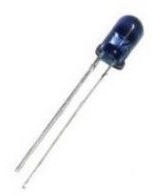
\includegraphics[width=0.25\textwidth]{LEDInfrarrojo}
            \end{wrapfigure}

            Los LED infrarrojos son un tipo específico de diodo emisor de luz
            (LED por sus siglas en inglés) que produce luz en el espectro infrarrojo.
            La luz en este rango no es visible para el ojo humano, pero puede ser
            detectada por una variedad de dispositivos electrónicos, haciendo al LED
            ideal para objetos como controles remotos, donde el LED no necesita ser
            visto para funcionar.

            

        % ==============================================================
        % =================      CARACTERISTICAS      ==================
        % ==============================================================
        \vspace{2em}
        \subsubsection{Características}

            \begin{itemize}
                \item 
                    \textbf{Tamaño}

                    80\% de los LED producidos en el mundo tienen 5 mm de diámetro.
                    Los LED infrarrojos no son diferentes y la mayoría de ellos tiene
                    5 mm de diámetro.

                \item 
                    \textbf{Color}

                    A pesar de que la luz emitida por un LED infrarrojo no es visible
                    para el ojo desnudo, la mayoría de los LED infrarrojos tienen una
                    cubierta morada alrededor. Esto ayuda a transmitir el color correcto
                    de luz.

                \item
                    \textbf{Brillo}

                    El brillo de un LED se mide en miliwatts (mW). A pesar de que la
                    luminiscencia de un LED depende de la cantidad de energía con que
                    se alimente, la mayoría de los LED producen 20 mW de luz en su
                    punto máximo y cerca de 1 mW de luz a un nivel de operación promedio.

            \end{itemize}


    % ==============================================================
    % =============      FOTOTRANSISTOR           ==================
    % ==============================================================
    \clearpage
    \subsection{Fototransistor}

        % ==============================================================
        % =================      DEFINICION           ==================
        % ==============================================================
        \subsubsection{Definición}

            \begin{wrapfigure}{r}{0.35\textwidth}
                \centering
                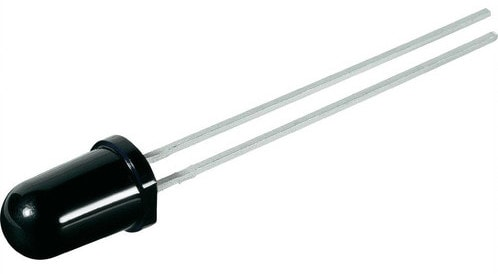
\includegraphics[width=0.30\textwidth]{Fototransistor}
            \end{wrapfigure}

            Un fototransistor es, en esencia, lo mismo que un transistor normal,
            sólo que puede trabajar maneras diferentes:

            \begin{itemize}
                \item Como un transistor normal con la corriente de base (IB) (modo común)
                \item Como fototransistor, cuando la luz que incide en este elemento hace
                    las veces de corriente de base. (IP) (modo de iluminación). 
            \end{itemize}

            Se pueden utilizar las dos en forma simultáneamente, aunque este componente
            se utiliza principalmente con la patita de la base sin conectar ($I_B$ = 0).

            La corriente de base total es igual a corriente de base (modo común) + corriente
            de base (por iluminación): $I_{BT} = I_B + I_P$.

            Este componente es muy utilizado en aplicaciones donde la detección de iluminación
            es muy importante. Como el fotodiodo, tiene un tiempo de respuesta muy corto, y si
            lo conectamos como se muestra en el diagrama anterior, tenemos un semiconductor de
            rápida respuesta a la iluminación y de gran capacidad de entrega de corriente.



    % ==============================================================
    % =================      FOTORESISTENCIA      ==================
    % ==============================================================
    \vspace{1em}
    \subsection{Sensor Infrarrojo}

        El sensor de infrarrojos es un sensor de medición de distancia, que se basa en un
        sistema de emisión/recepción de radiación lumínica en el espectro de los infrarrojos
        (menor que las ondas de radio y mayor que la luz).

        Una de las técnicas más habituales para la medición de la distancia es mediante la
        triangulación del haz de luz colimada, si bien también se puede "estimar" la distancia
        de un objeto a partir de la cantidad de energía recibida tras rebotar la luz sobre un objeto.

        En robótica móvil se suelen utilizar sensores baratos de corto alcance, en un rango máximo
        de unos 50/80 cm. y el tipo de detección que realizan es direccional, es decir, sólo son
        capaces de detectar objetos que están enfrente del sensor.

        Este tipo de sensor presenta el inconveniente de ser sensible a la luz ambiente como
        consecuencia de que los rayos de sol también emiten en el espectro de luz infrarroja.
        Por este motivo, son sensores que se utilizan habitualmente en entornos con iluminación
        artificial de forma predominante (interiores).

        % ==============================================================
        % =================        ESTRUCTURA         ==================
        % ==============================================================
        \subsubsection{Estructura}

            \begin{wrapfigure}{r}{0.30\textwidth}
                \centering
                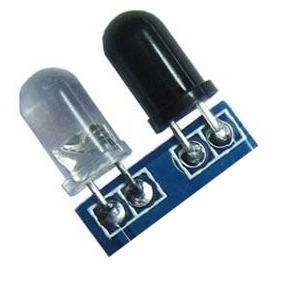
\includegraphics[width=0.30\textwidth]{SensorInfrarrojo}
            \end{wrapfigure}

            Como se puede apreciar en la imagen, el consta de
            un LED Infrarrojo y un fototransistor.

            Vamos a colocarlos, de tal manera que usemos un principio conocido
            como medición por triangulación.


        % ==============================================================
        % ========     FUNCIONAMIENTO FISICO          ==================
        % ==============================================================
        \subsection{Triangulación}

            El sensor infrarrojo funciona mediante el principio de triangulación
            de la luz que rebota sobre el objeto (de forma no especular).

            Tal y como se aprecia en la siguiente figura, el haz de luz incide con
            un ángulo diferente en función de la distancia del sensor.
            Este ángulo de incidencia es captado por una película lineal fotosensible
            que proporciona un valor analógico a la salida en función de la posición
            en la que el rayo de luz impacta.


            Se puede fácilmente apreciar que uno de las principales inconvenientes de
            esta técnica de medición es que el ángulo de incidencia apenas varía para
            grandes distancias, con lo que el sensor es poco sensible para grandes
            distancias como se verá a continuación.


            \begin{figure}[h]
                \centering
                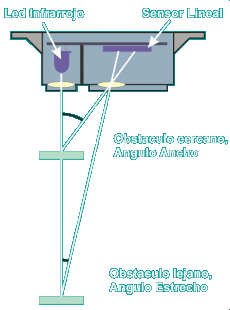
\includegraphics[width=0.4\textwidth]{Triangulacion}
            \end{figure}




% ===============================================================================
% ===================          DESARROLLO                  ======================
% ===============================================================================
\clearpage
\section{Desarrollo}


    % ==============================================================
    % =================      DIAGRAMAS            ==================
    % ==============================================================
    \subsection{Diagramas}

        Veamos que nuestro circuito puede ser descrito con el siguiente diagrama:
        \begin{figure}[h]
            \centering
            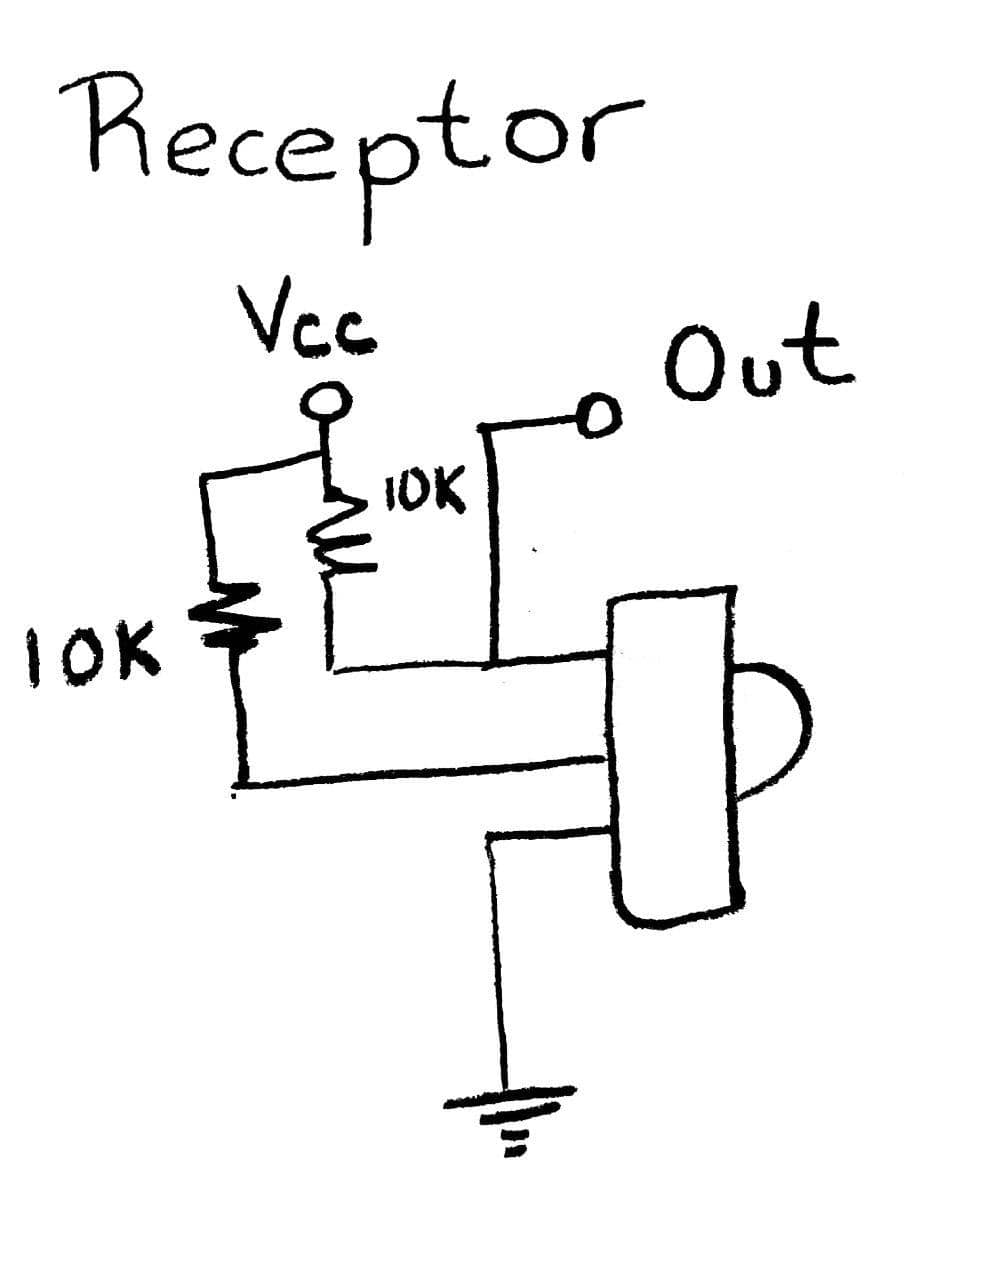
\includegraphics[width=0.4\textwidth]{Diagram0}
            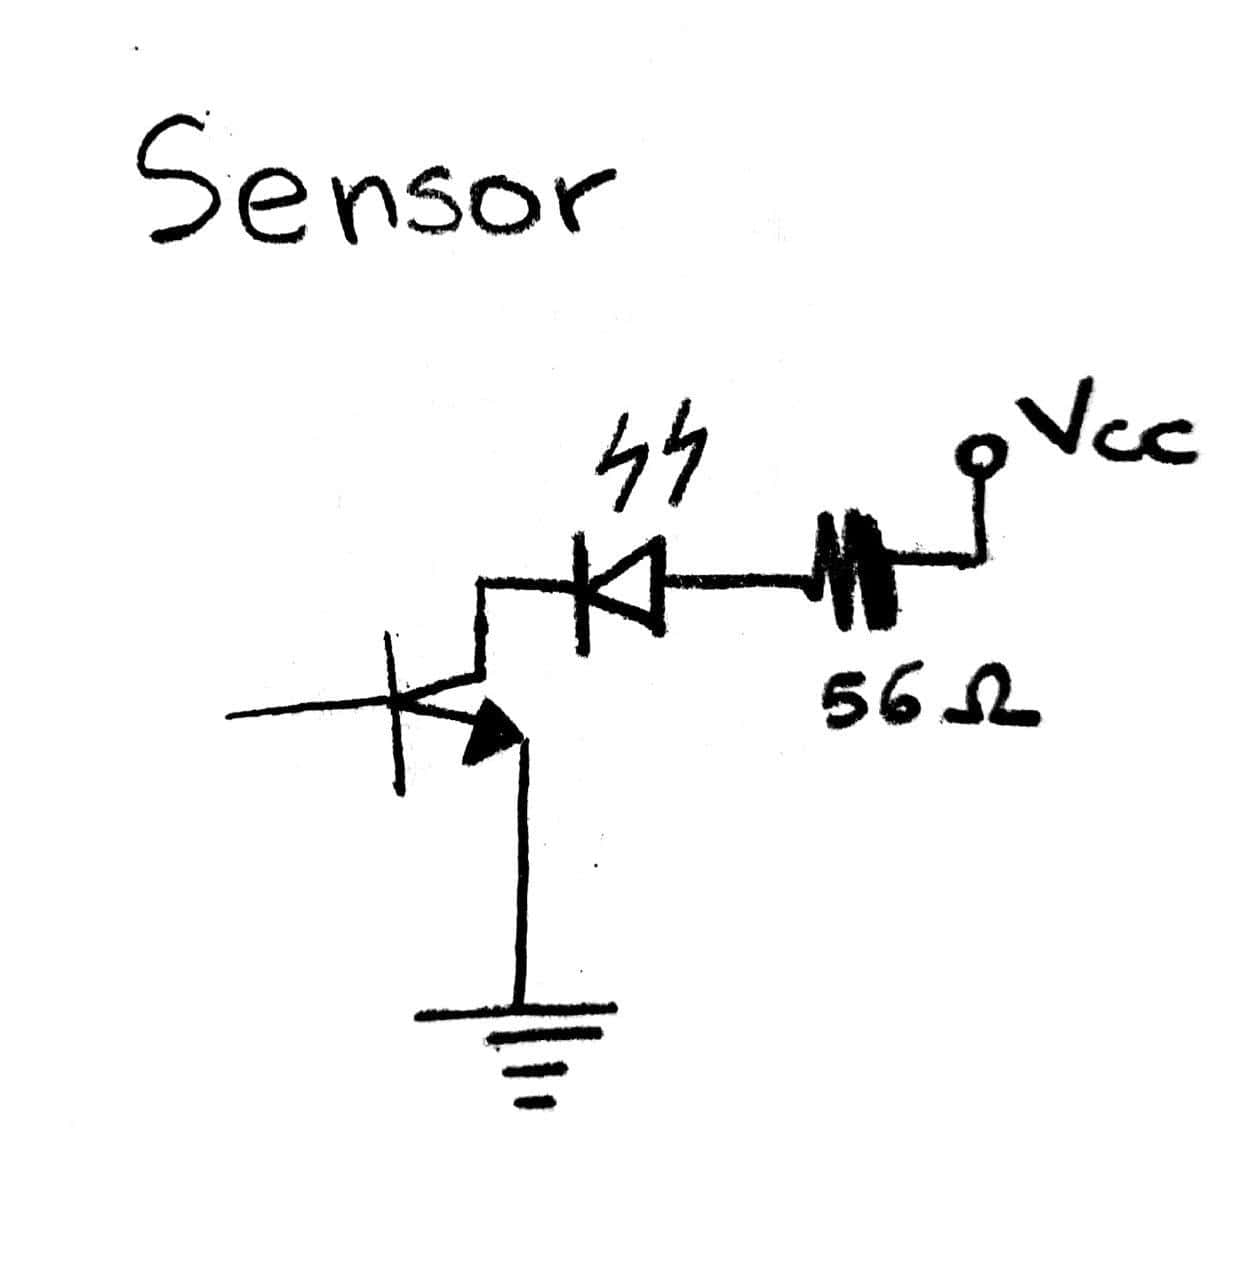
\includegraphics[width=0.4\textwidth]{Diagram1}
        \end{figure}

        Este lo podemos dividir basicamente en 2 partes:
        \begin{itemize}
            \item 
                \textbf{Circuito Sensor}

                Lo que haciamos es en la parte de la señal infrarroja era
                fáil, simplemente usando un transistor para poder accionar
                el flujo de la corriente facilmente, poniendo un resistor
                realmente pequeño pero que era la clave para que en los pequeños
                pulsos o impulsos nuestro LED alcanzará una gran luminisencia.
            \item 
                \textbf{Circuito Receptor}

                Lo que hicimos fue seguir las especificaciones, y conectar a la salida un osciloscopio
                que nos permitiera medir el resultado de nuestra señal para calibrarlo

        \end{itemize}


    % ==============================================================
    % =================      CIRCUITO REAL        ==================
    % ==============================================================
    \clearpage
    \subsection{Modulación}

        Dedido a que nuestro LED no podria dar un gran brillo sin que tuvieramos que hacerle pasar
        una alta corriente y por lo tanto quemarlo, usamos modulación para poder hacer que nuestro circuito
        pudiera funcionar incluso a grandes distancias (casi un metro).

        Lo que hicimos fue generar una señal con una alta frecuencia, importante, la frecuencia
        es importante, esta tiene un punto clave en el que funciona, dicho punto o frecuencia
        especial depende del sensor, en nuestro caso estando alrededor de los 38 KHz

        \begin{figure}[h]
            \centering
            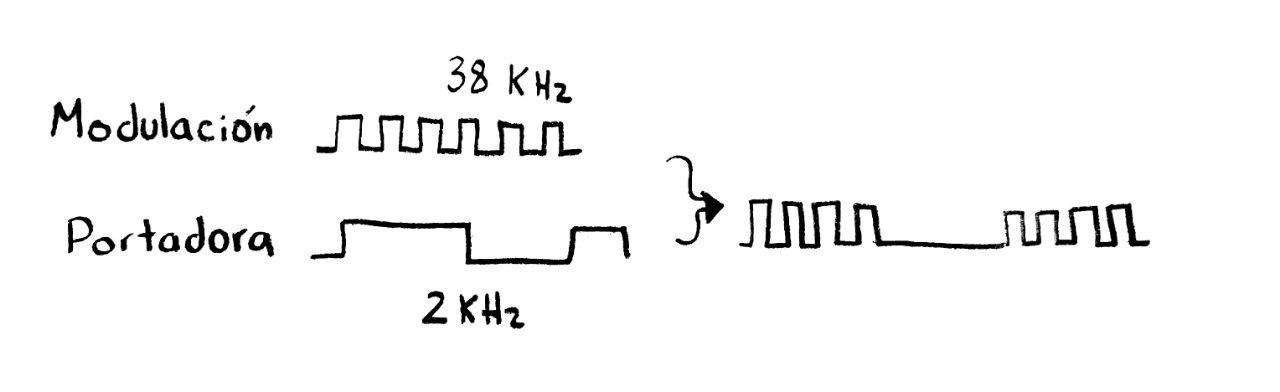
\includegraphics[width=0.85\textwidth]{Diagram2}
        \end{figure}

  

    % ==============================================================
    % =================      CIRCUITO REAL        ==================
    % ==============================================================
    \vspace{1em}
    \subsection{Circuito Real}

        Veamos que nuestro circuito fue construido de la siguiente manera:
        \begin{figure}[h]
            \centering
            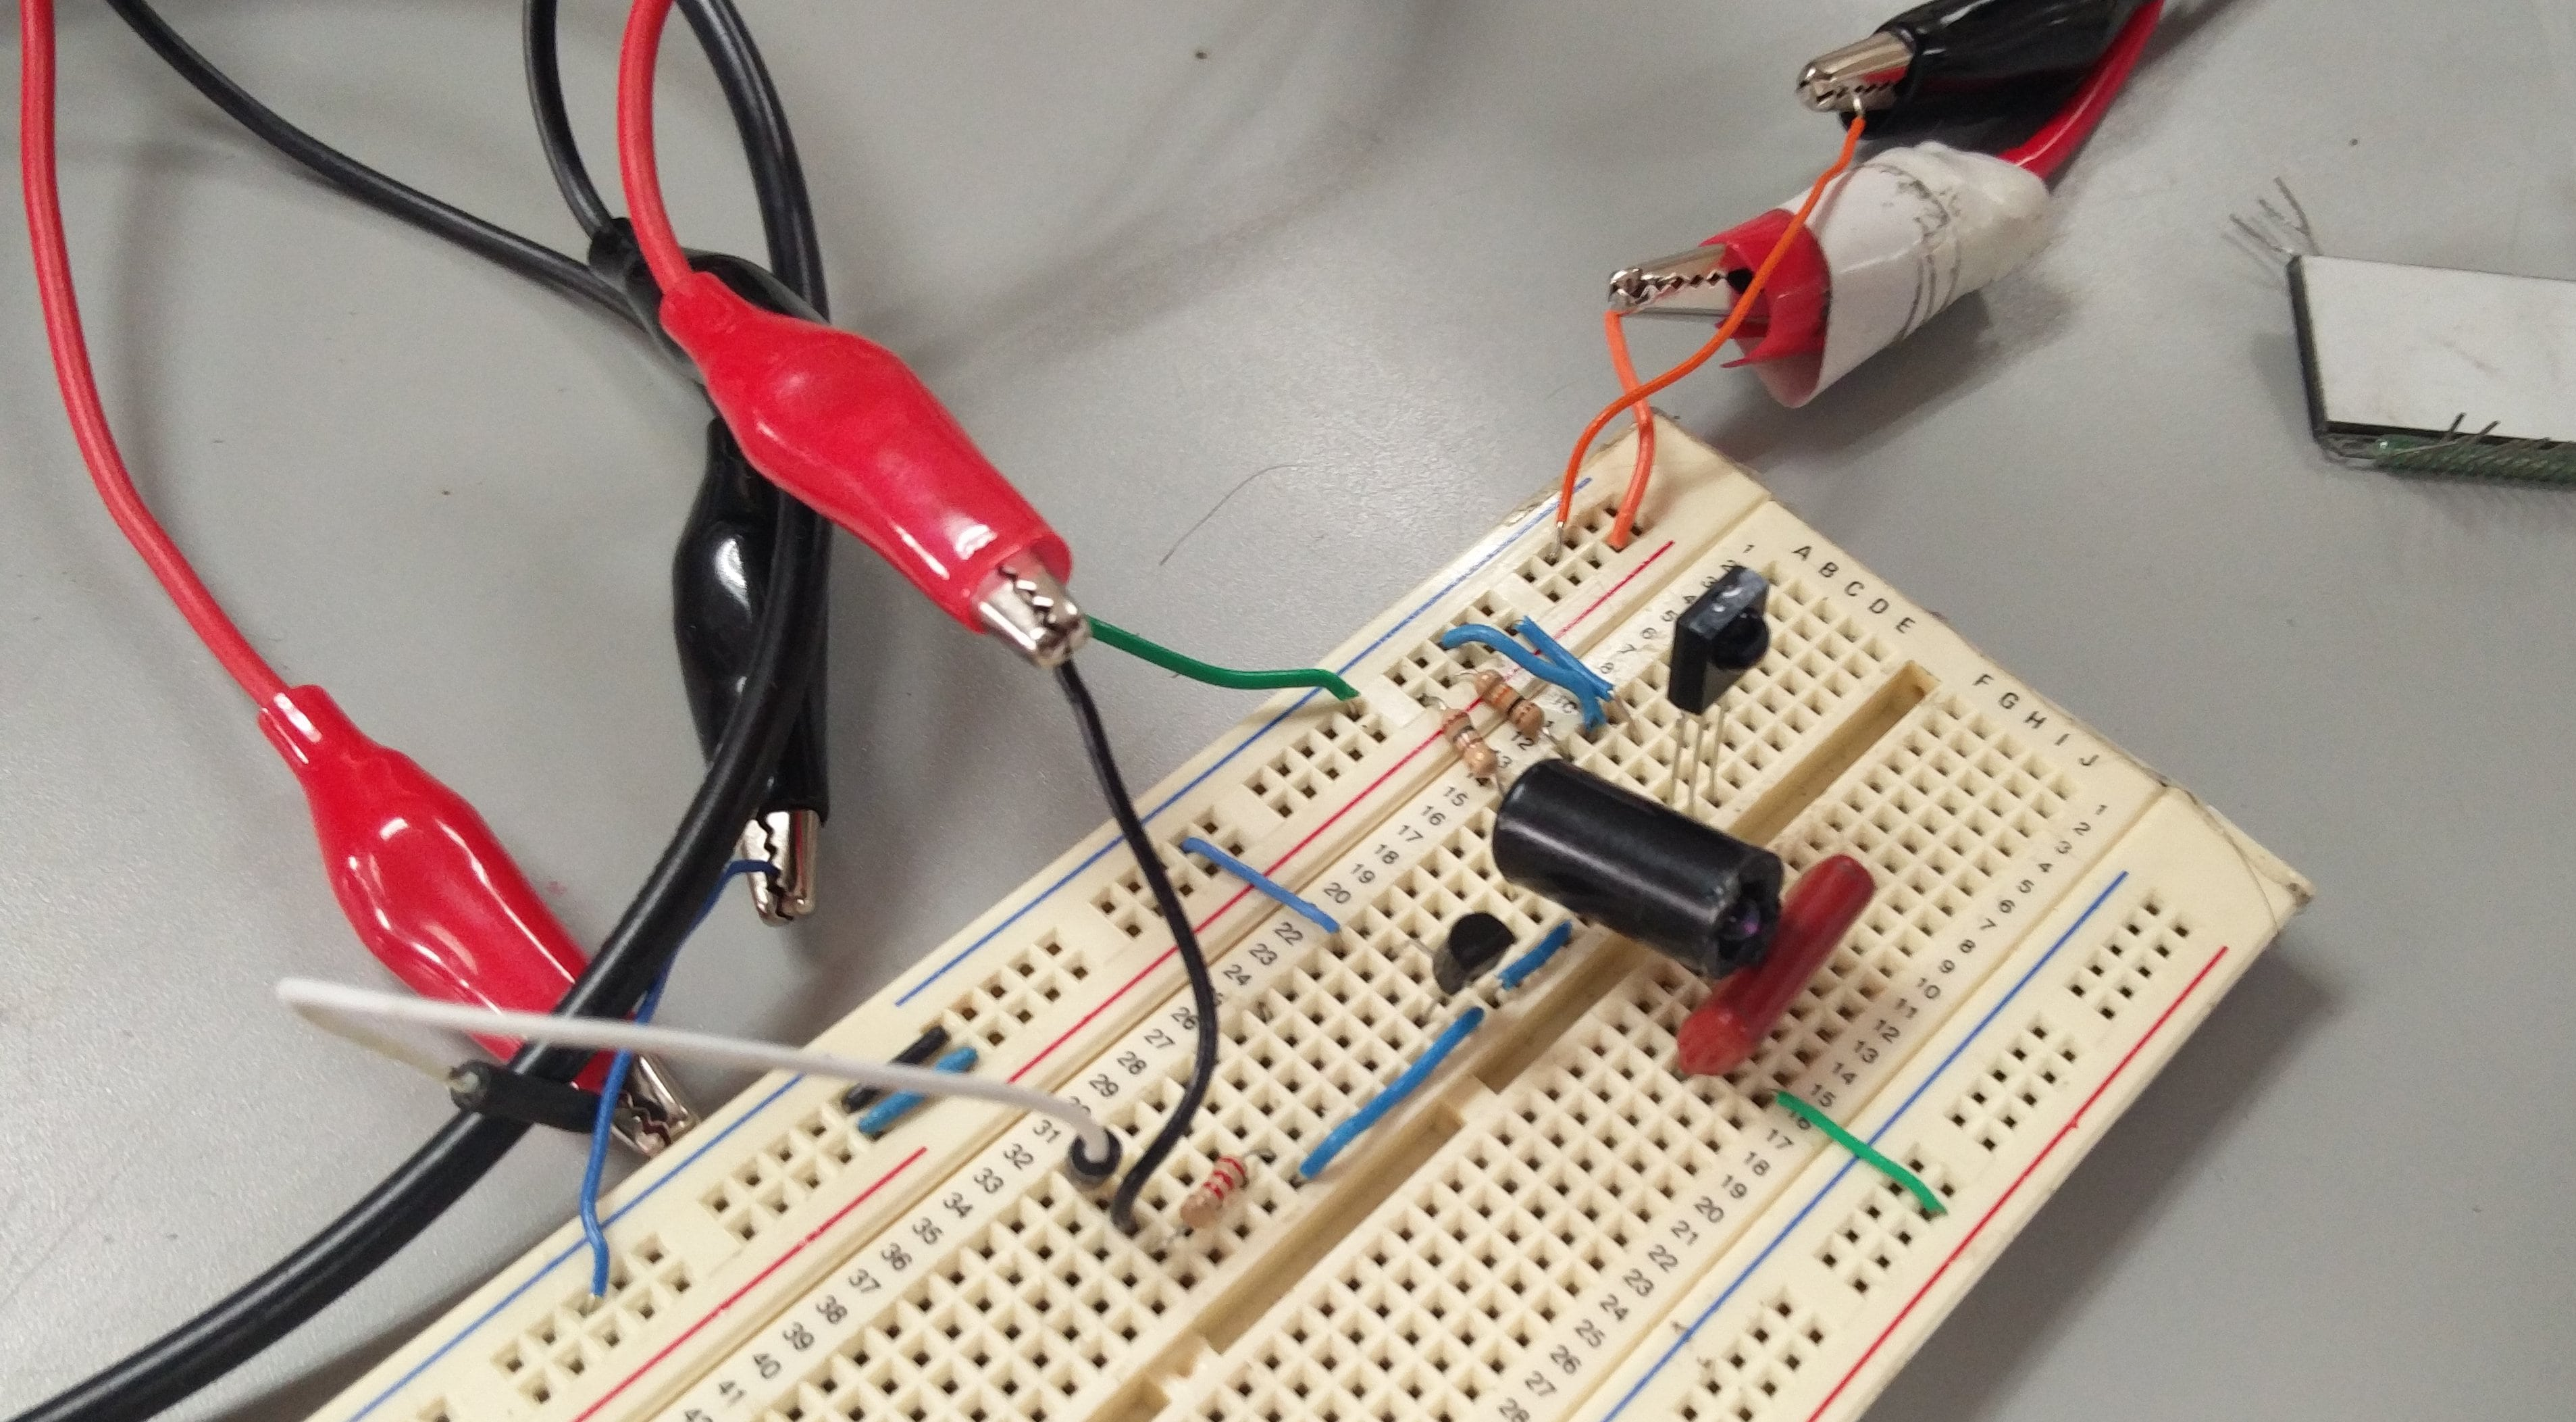
\includegraphics[width=0.85\textwidth]{CircuitoGeneral1}
        \end{figure}


    % ==============================================================
    % ================      CONFIGURACION SEÑAL      ===============
    % ==============================================================
    \clearpage
    \subsection{Configuración de la Señal Portadora}

        \begin{figure}[h]
            \centering
            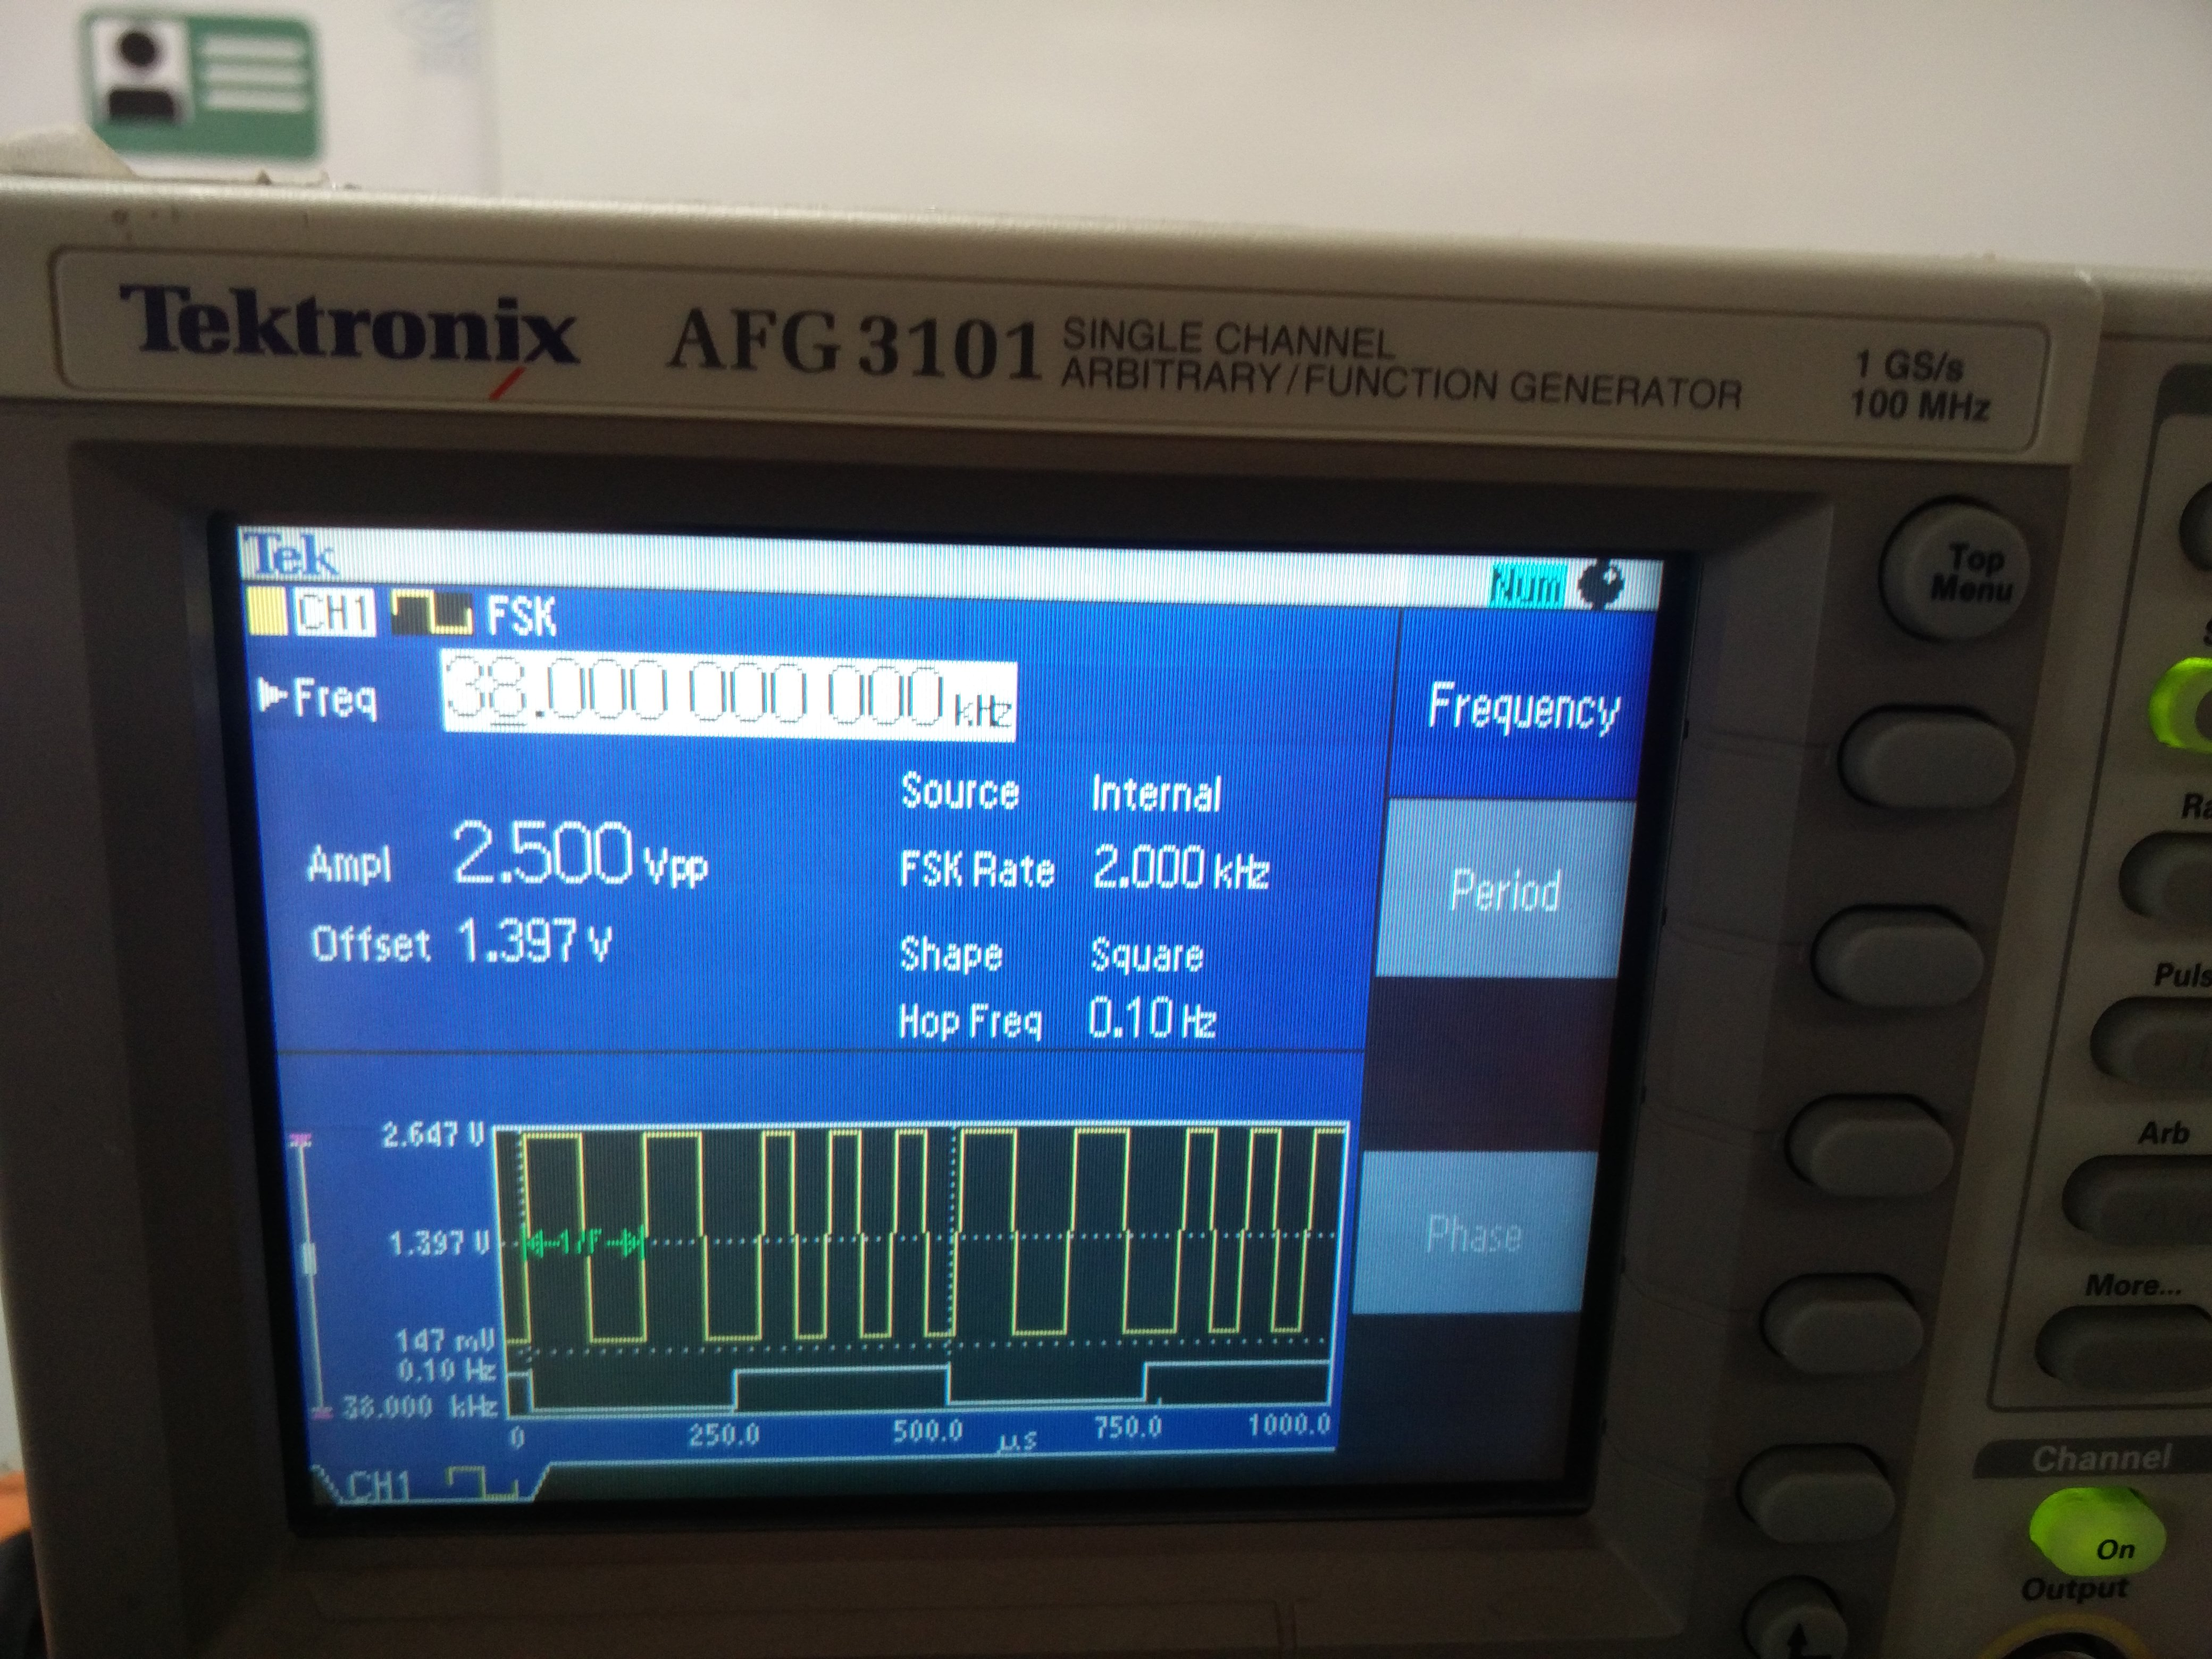
\includegraphics[width=0.6\textwidth]{Signal1}
            \caption{Configuración del Generador de Señales}
        \end{figure}

        \begin{figure}[h]
            \centering
            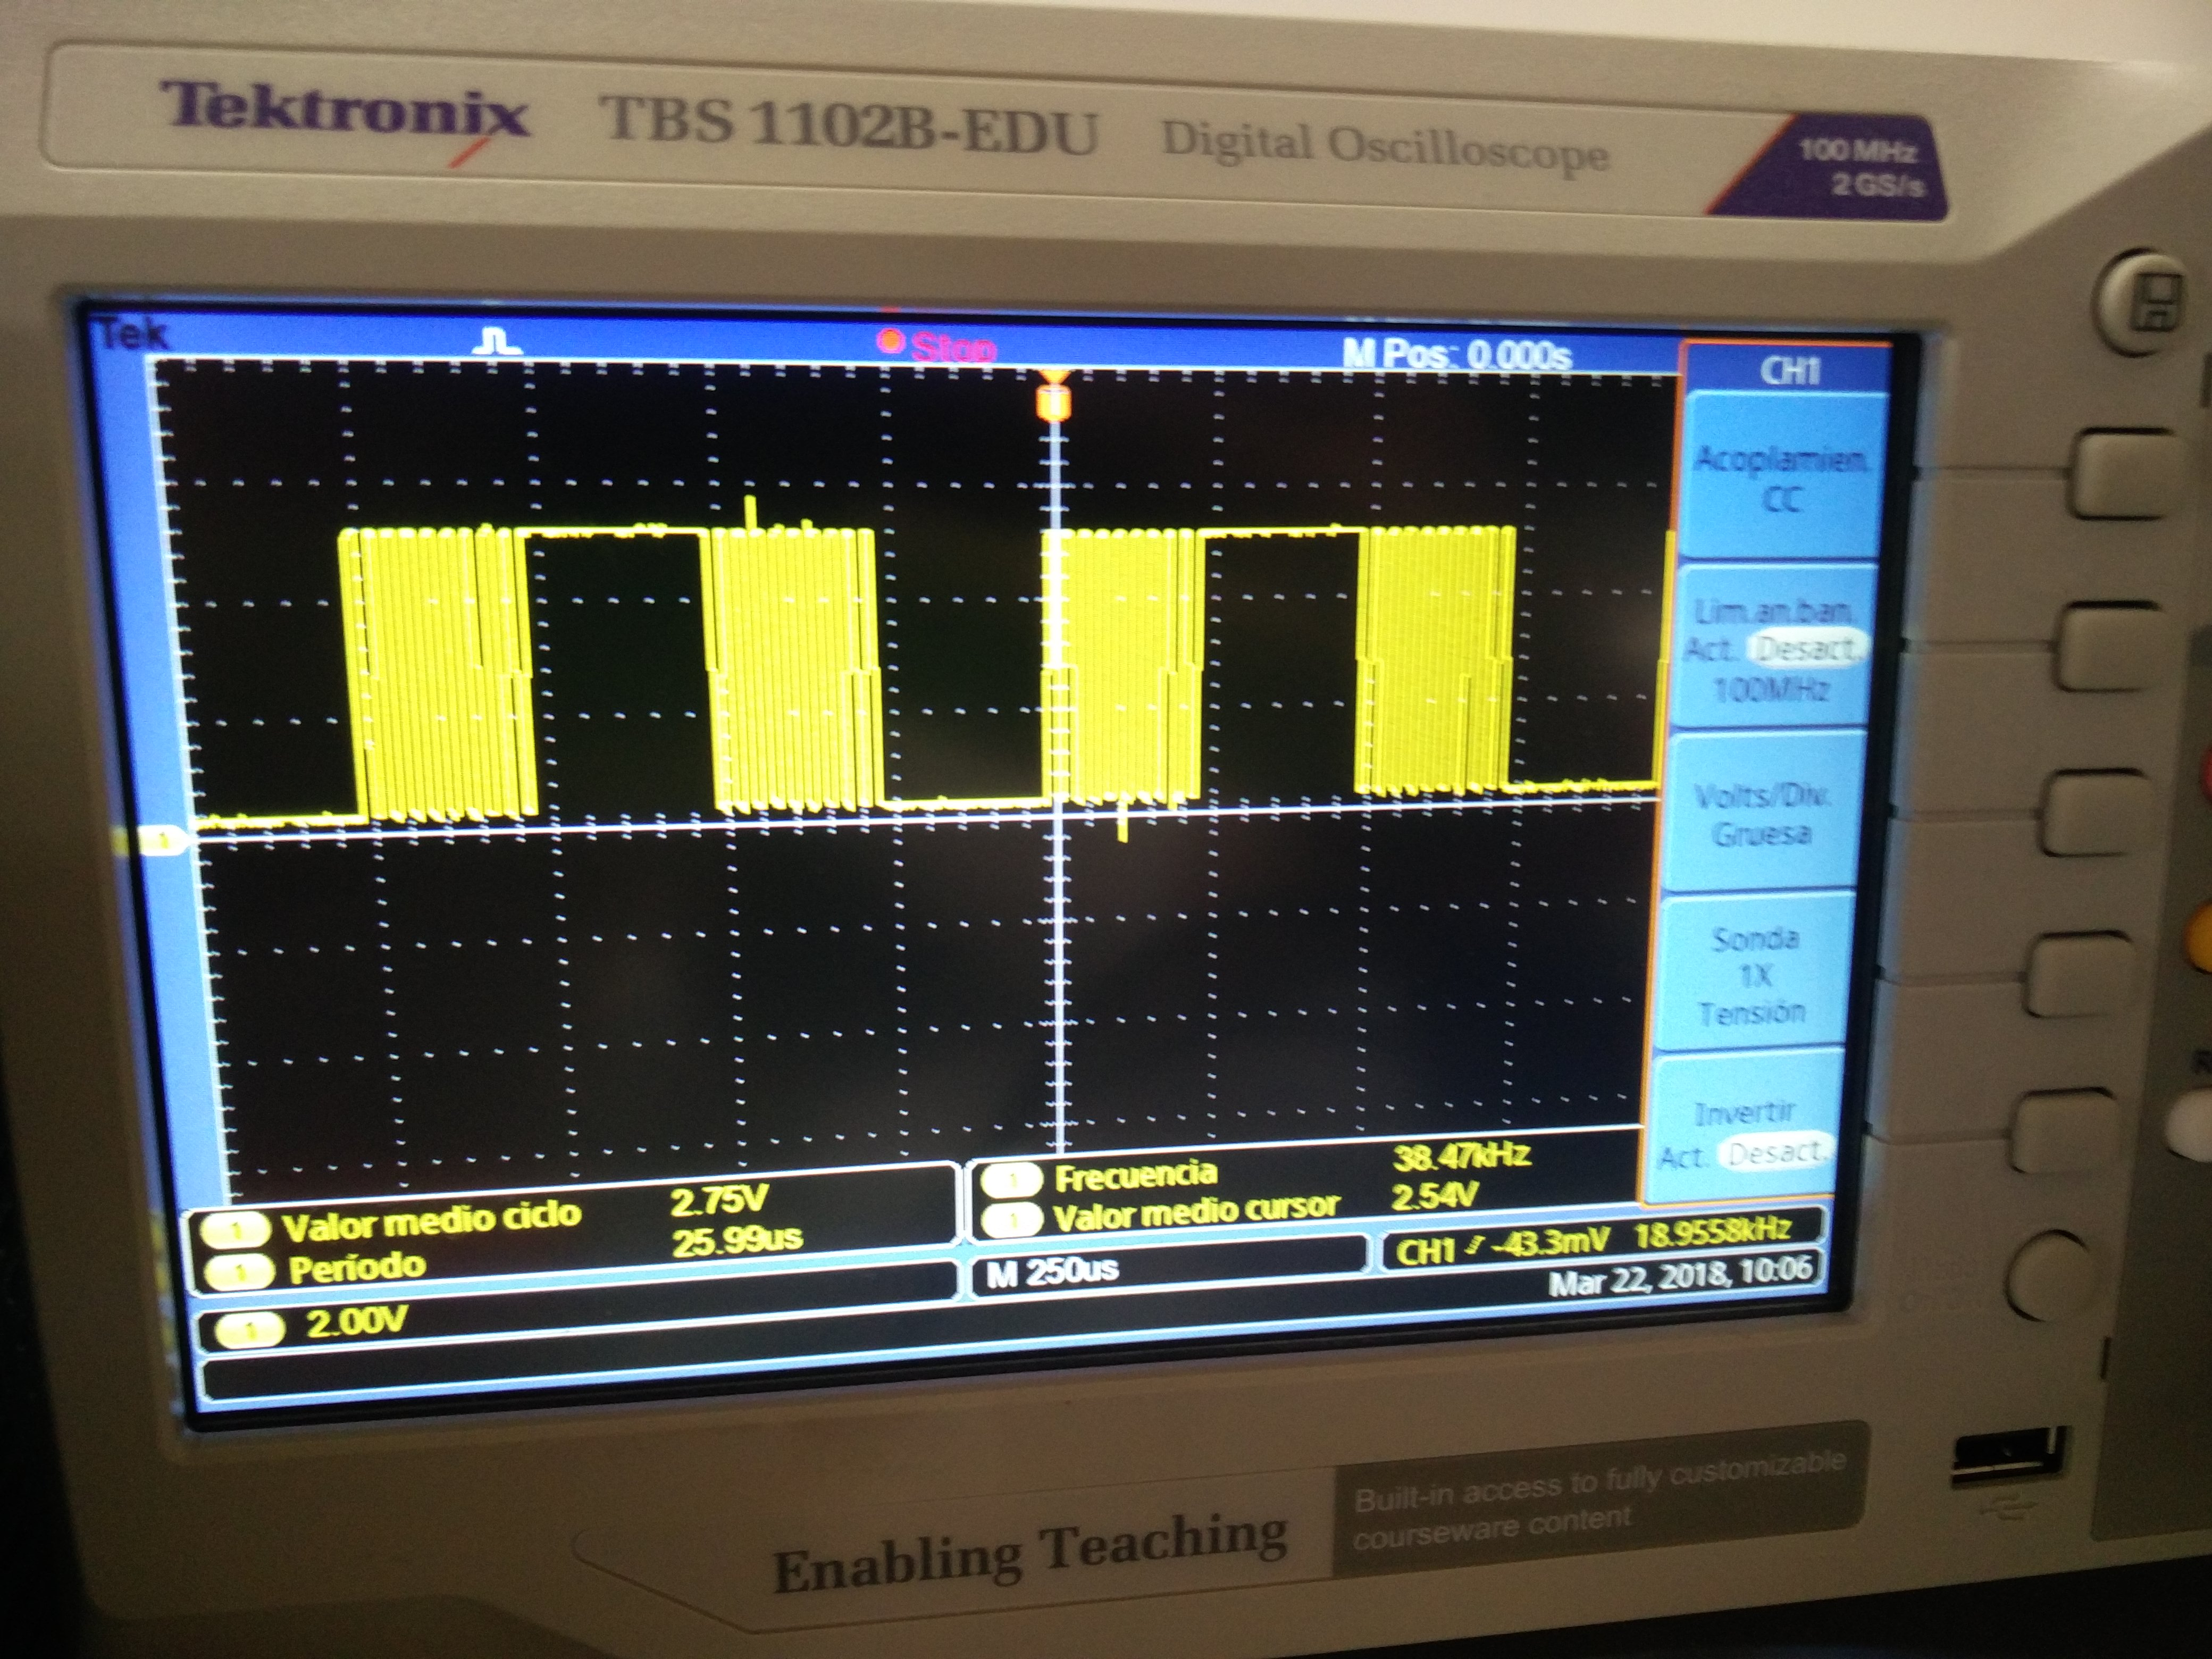
\includegraphics[width=0.6\textwidth]{Signal2}
            \caption{Forma de la señal}
        \end{figure}


    % ==============================================================
    % =================      MEDICIONES           ==================
    % ==============================================================
    \clearpage
    \subsection{Medición de Distancia}

        $\sim$ 2 cm de Distancia
        \begin{figure}[h]
            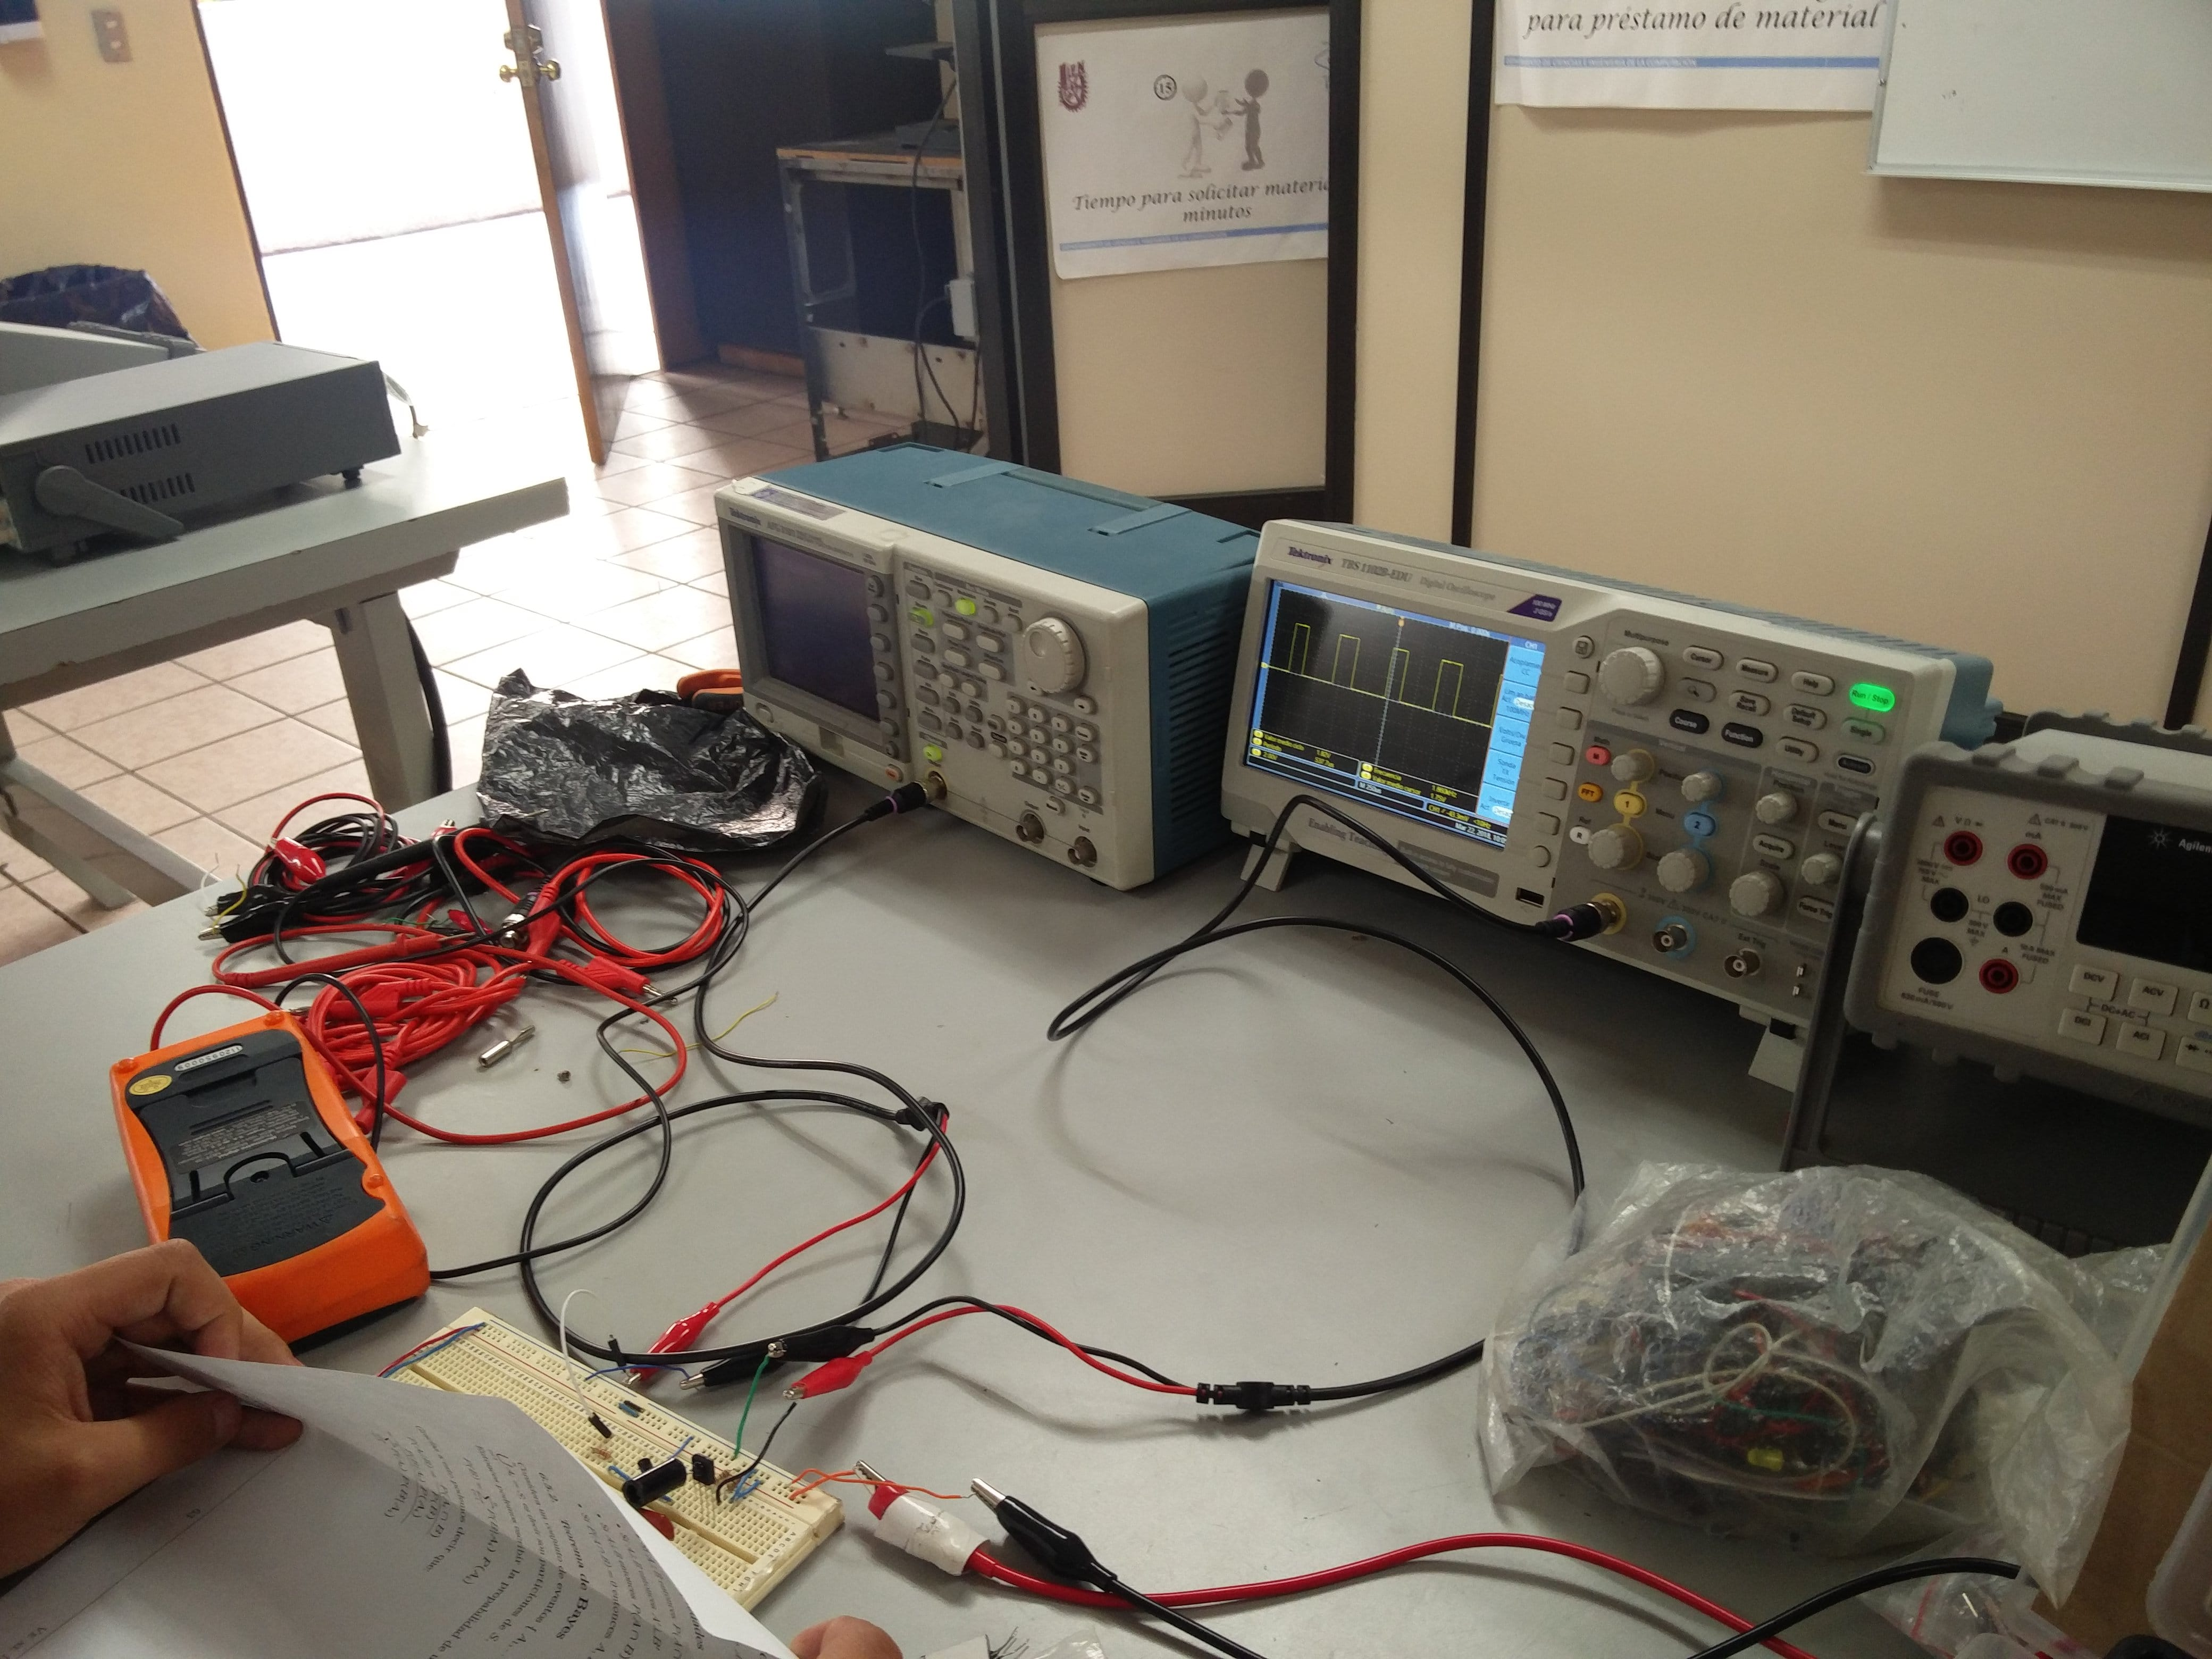
\includegraphics[width=0.4\textwidth]{1Distance}
            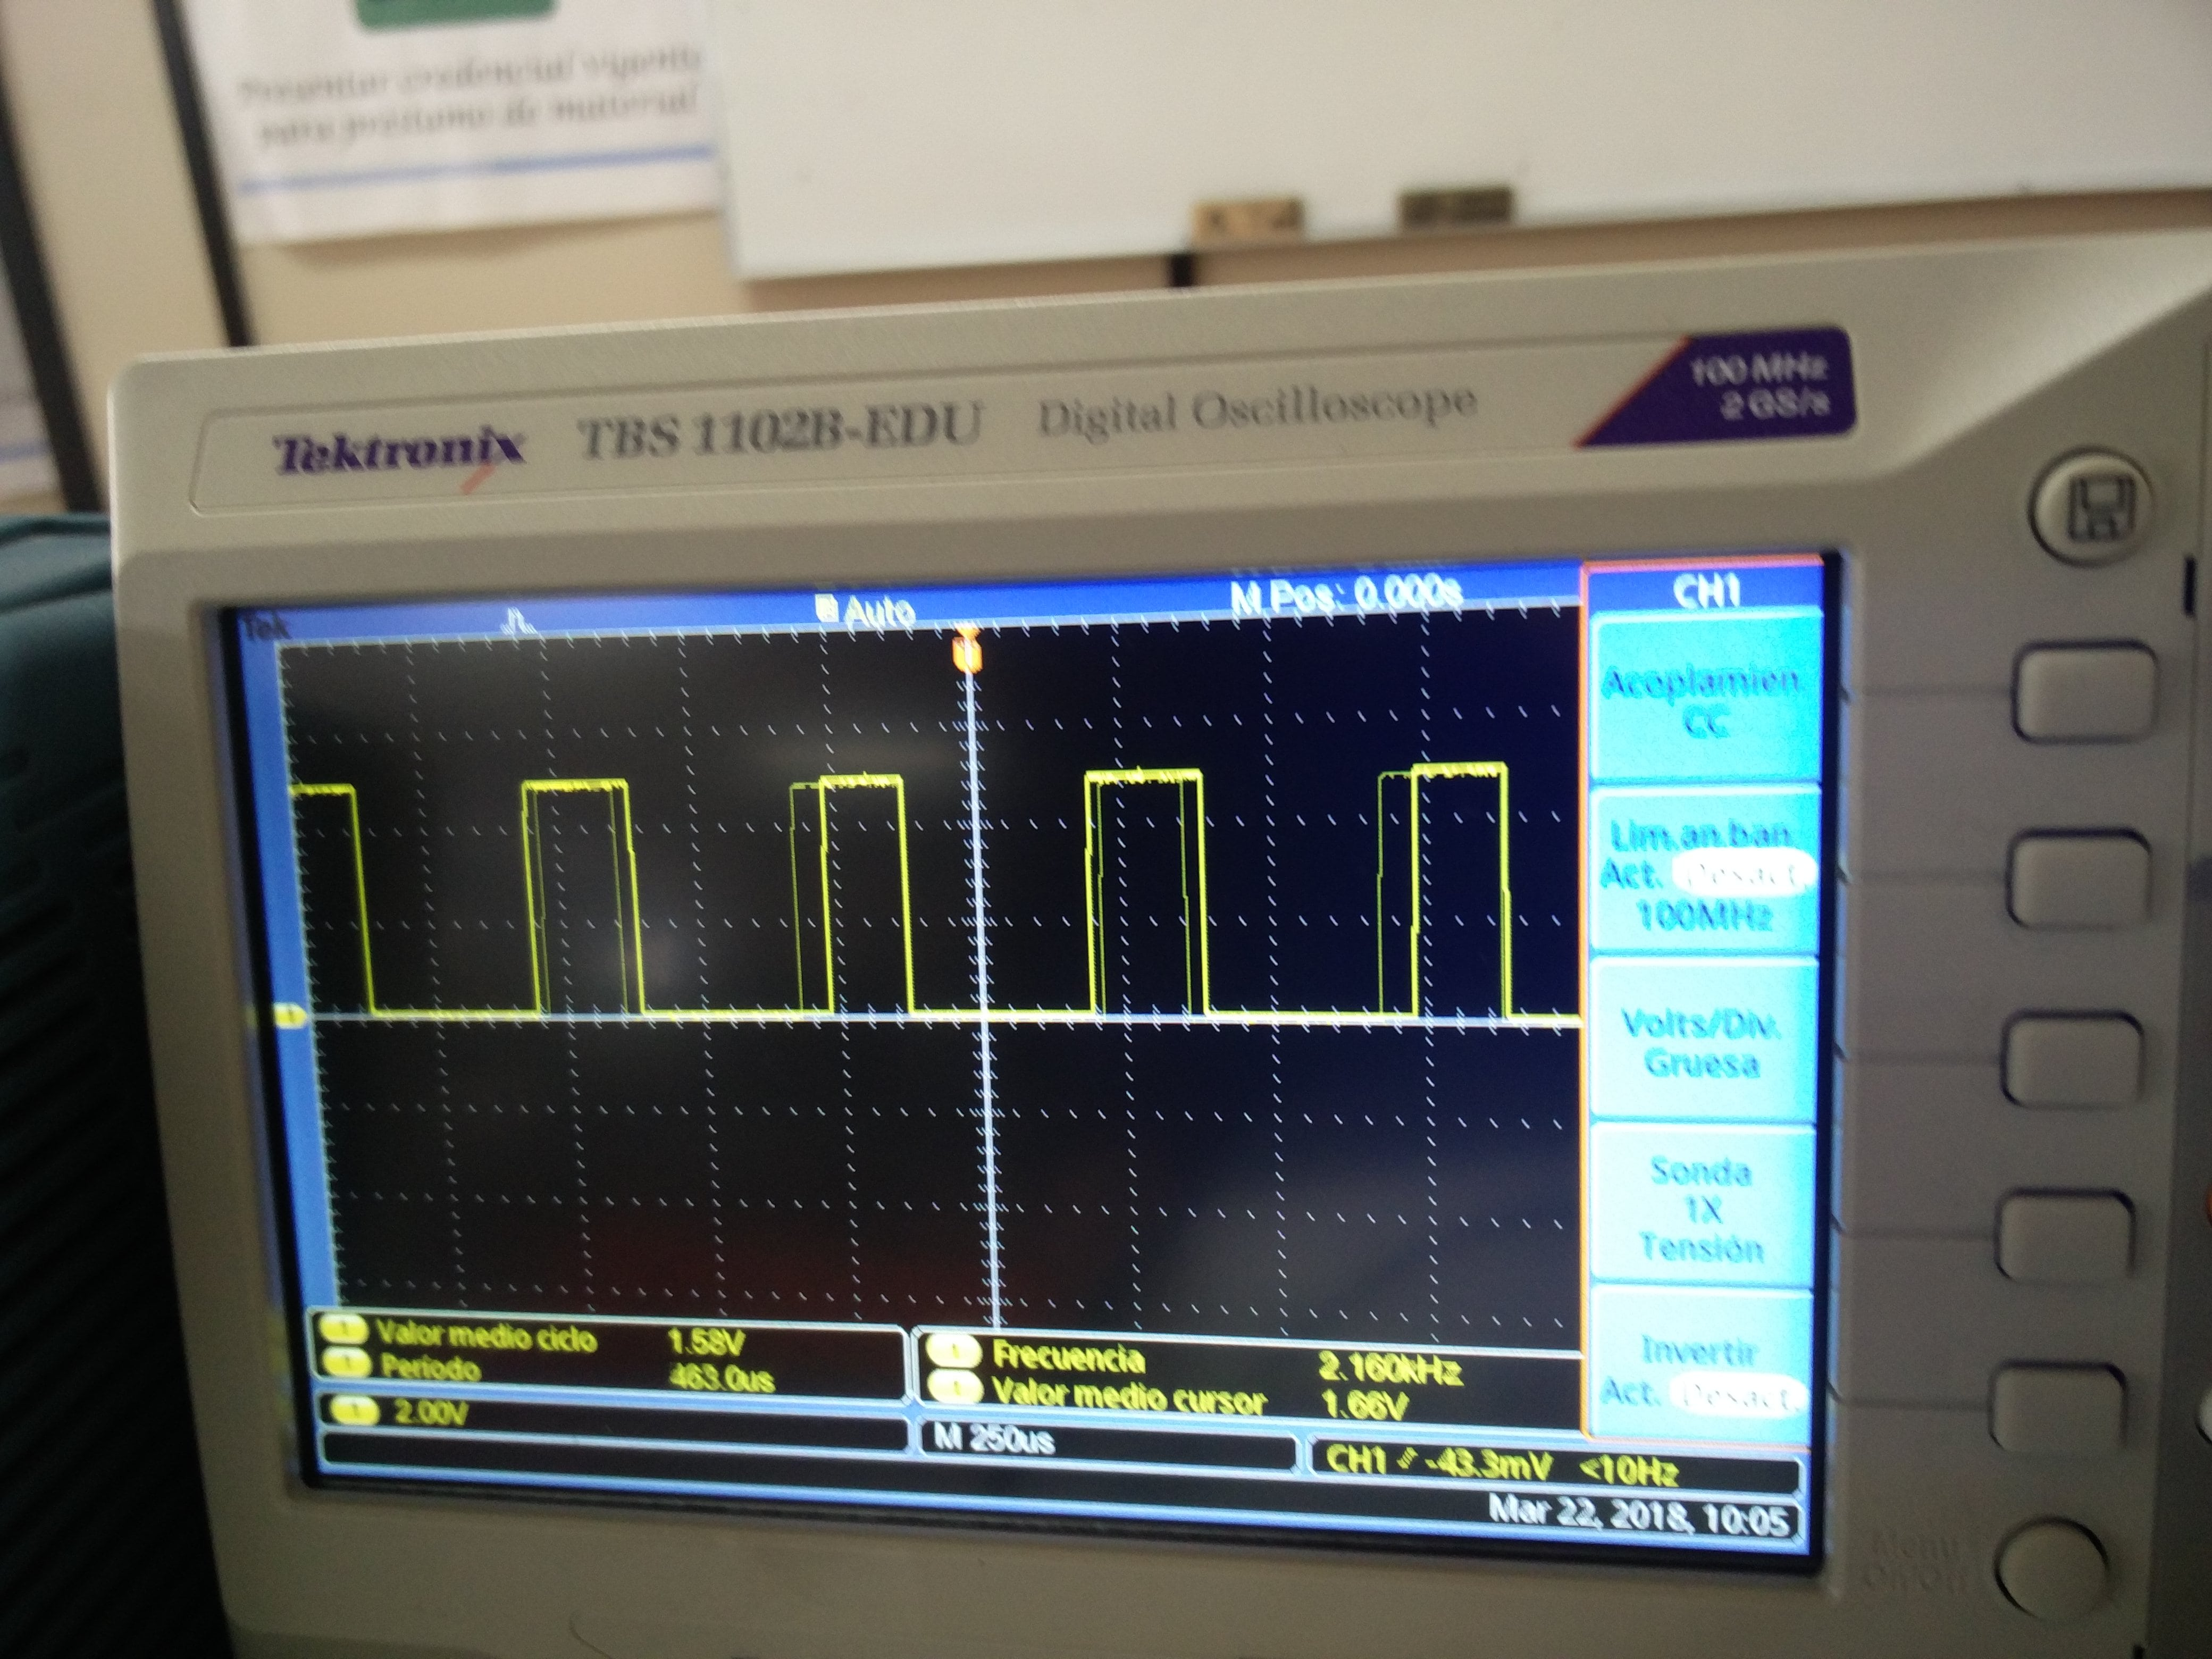
\includegraphics[width=0.4\textwidth]{1Signal}
        \end{figure}

        $\sim$ 5 cm de Distancia
        \begin{figure}[h]
            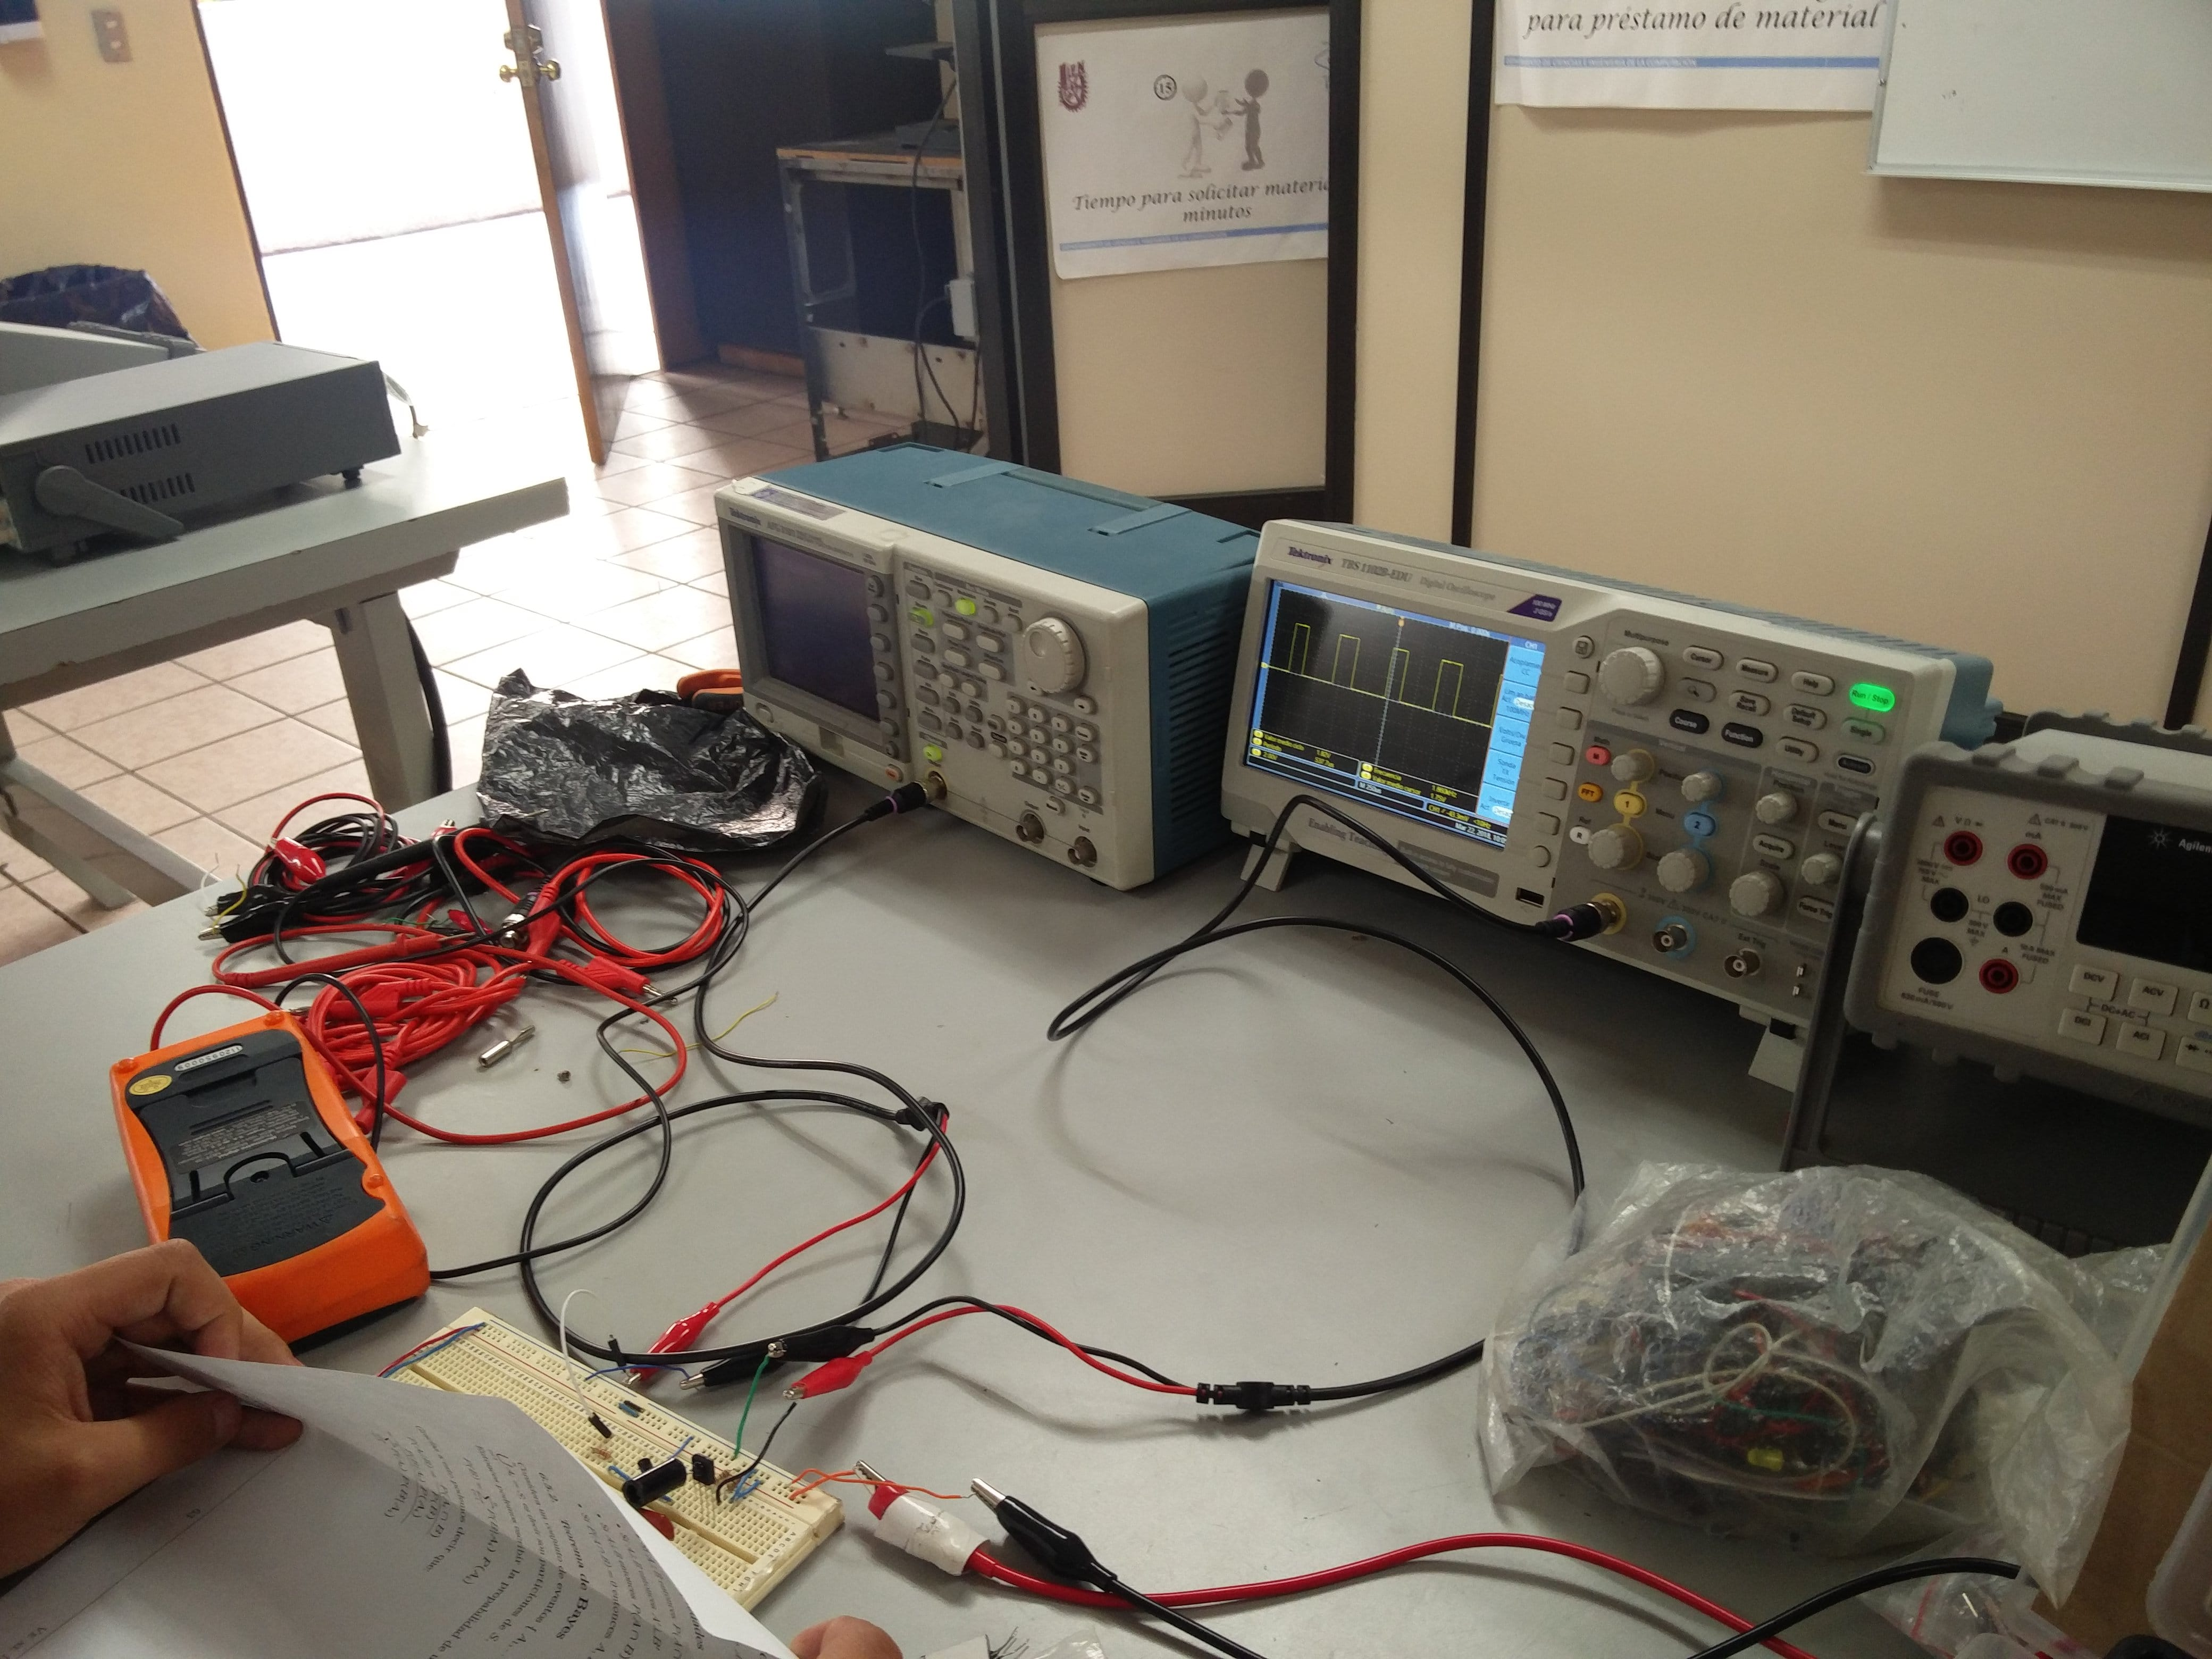
\includegraphics[width=0.4\textwidth]{3Distance}
            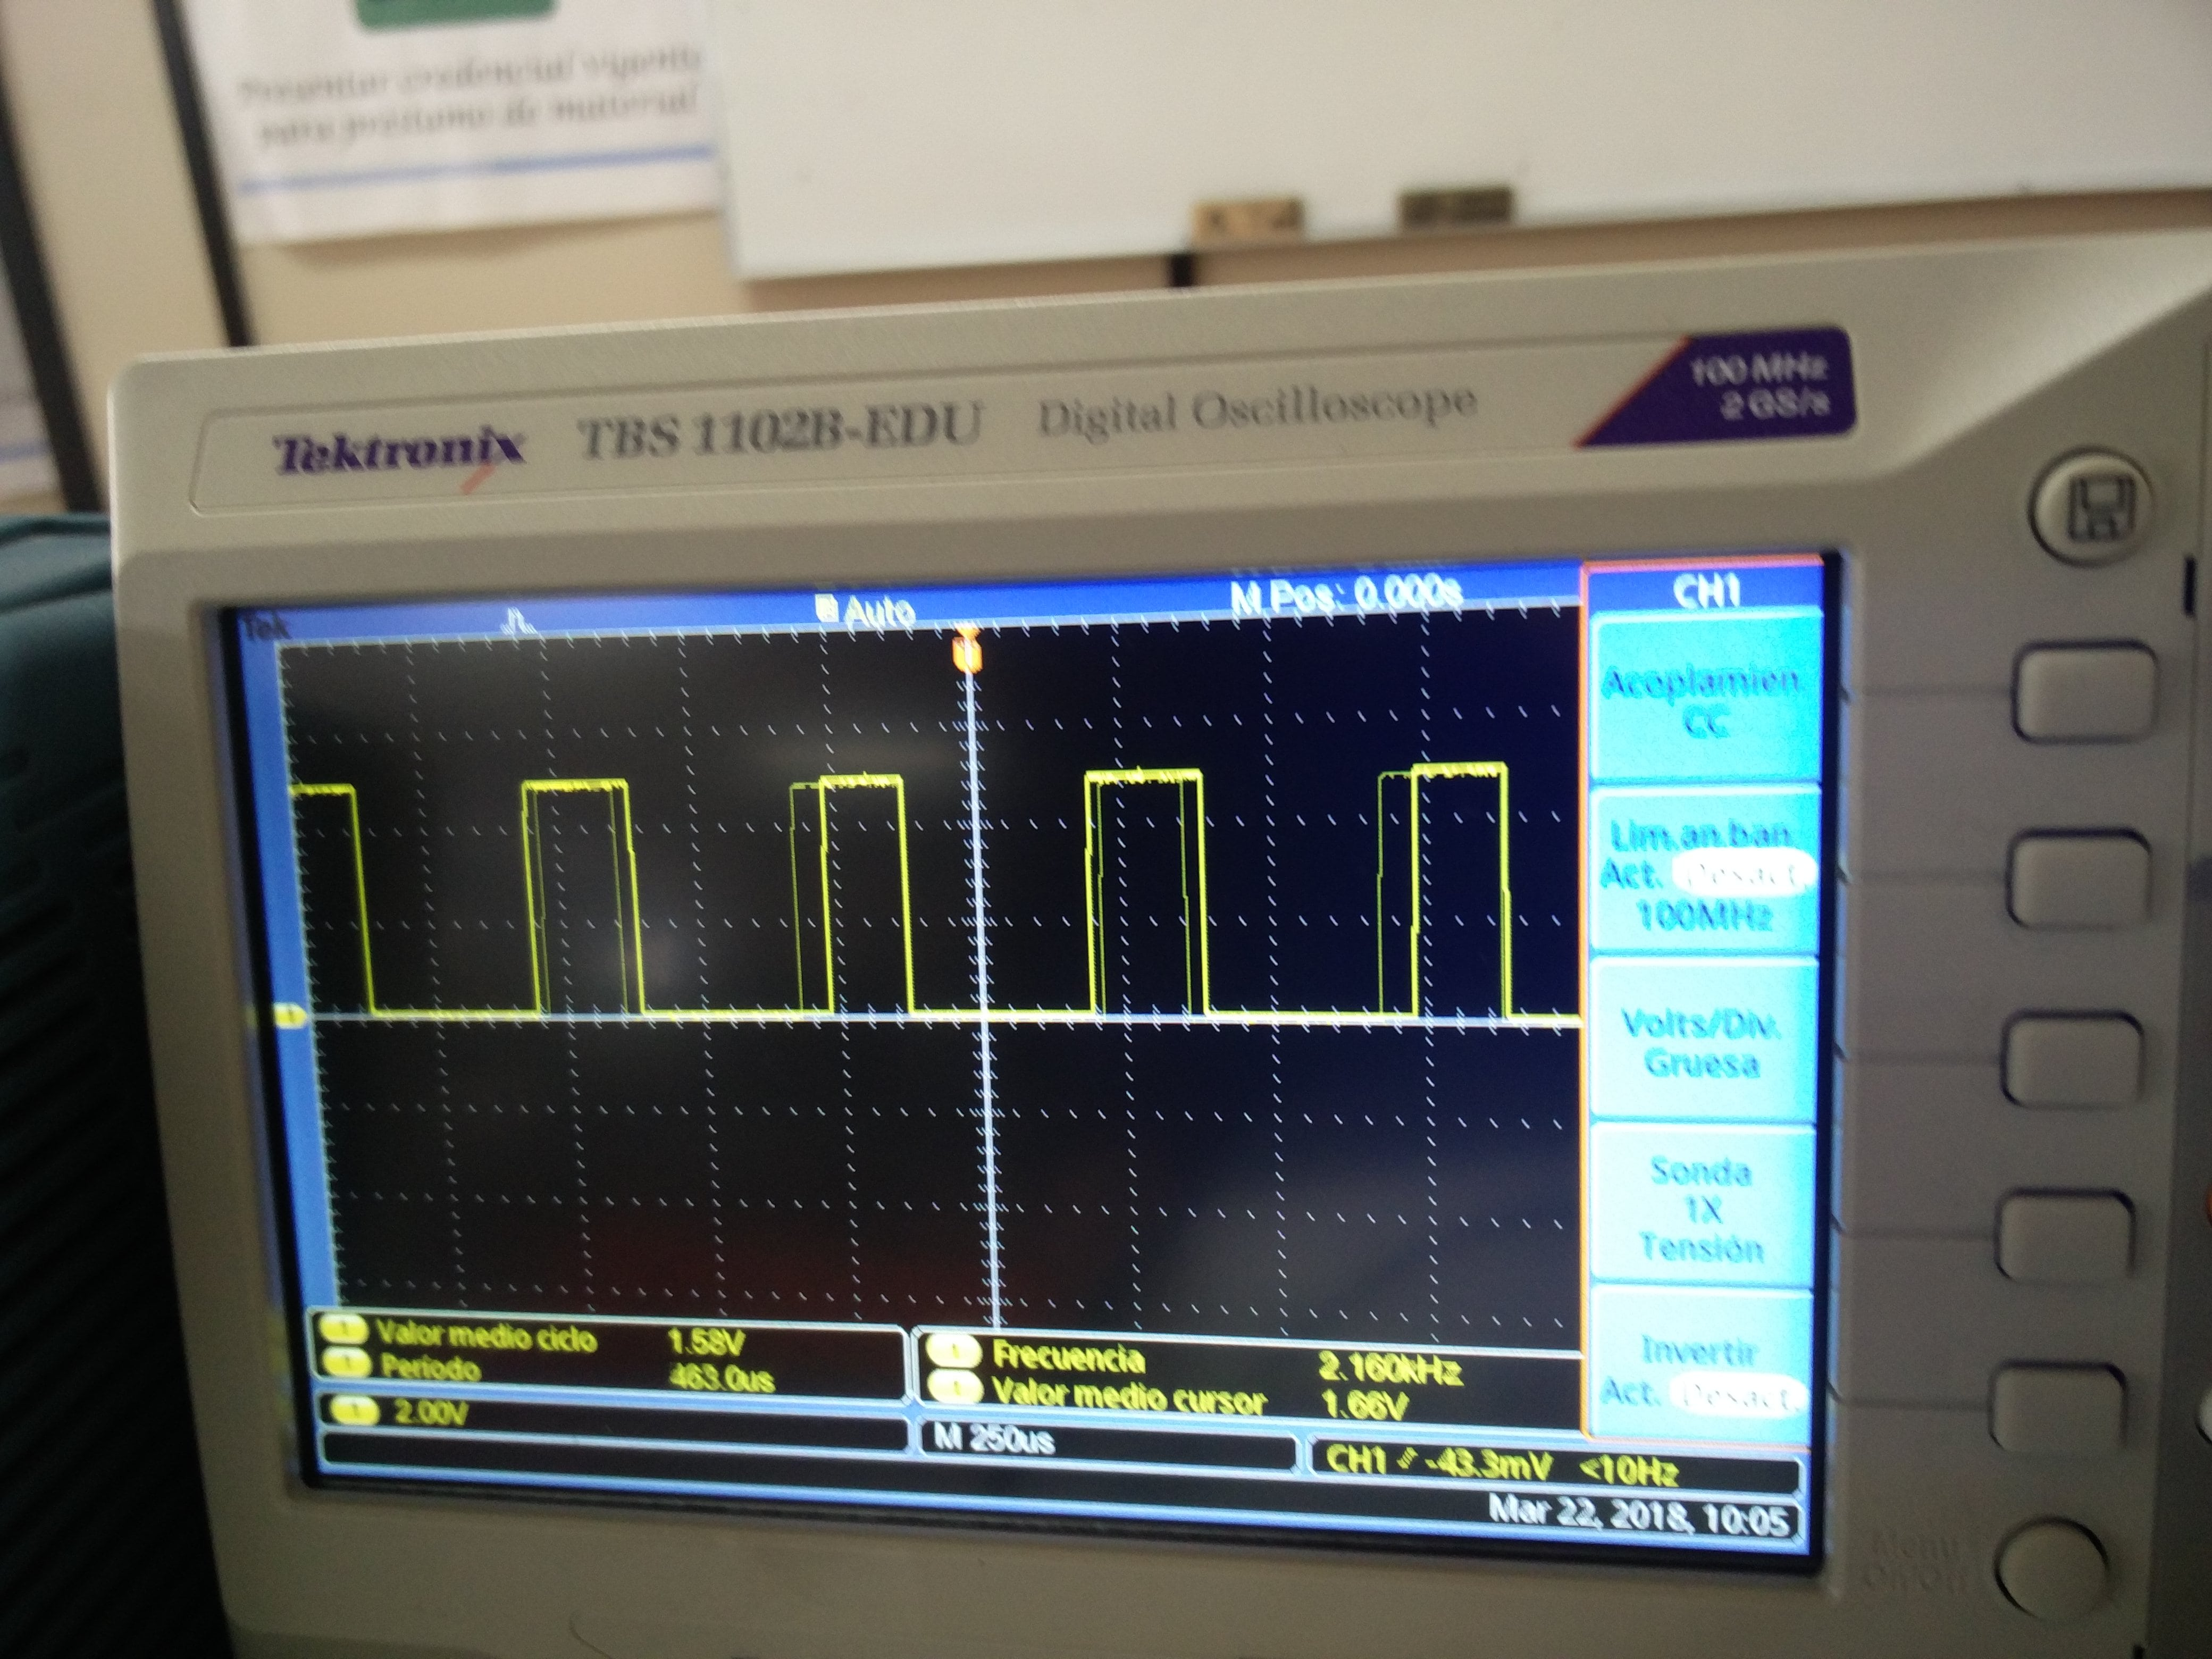
\includegraphics[width=0.4\textwidth]{3Signal}
        \end{figure}


        $\sim$ 20 cm de Distancia
        \begin{figure}[h]
            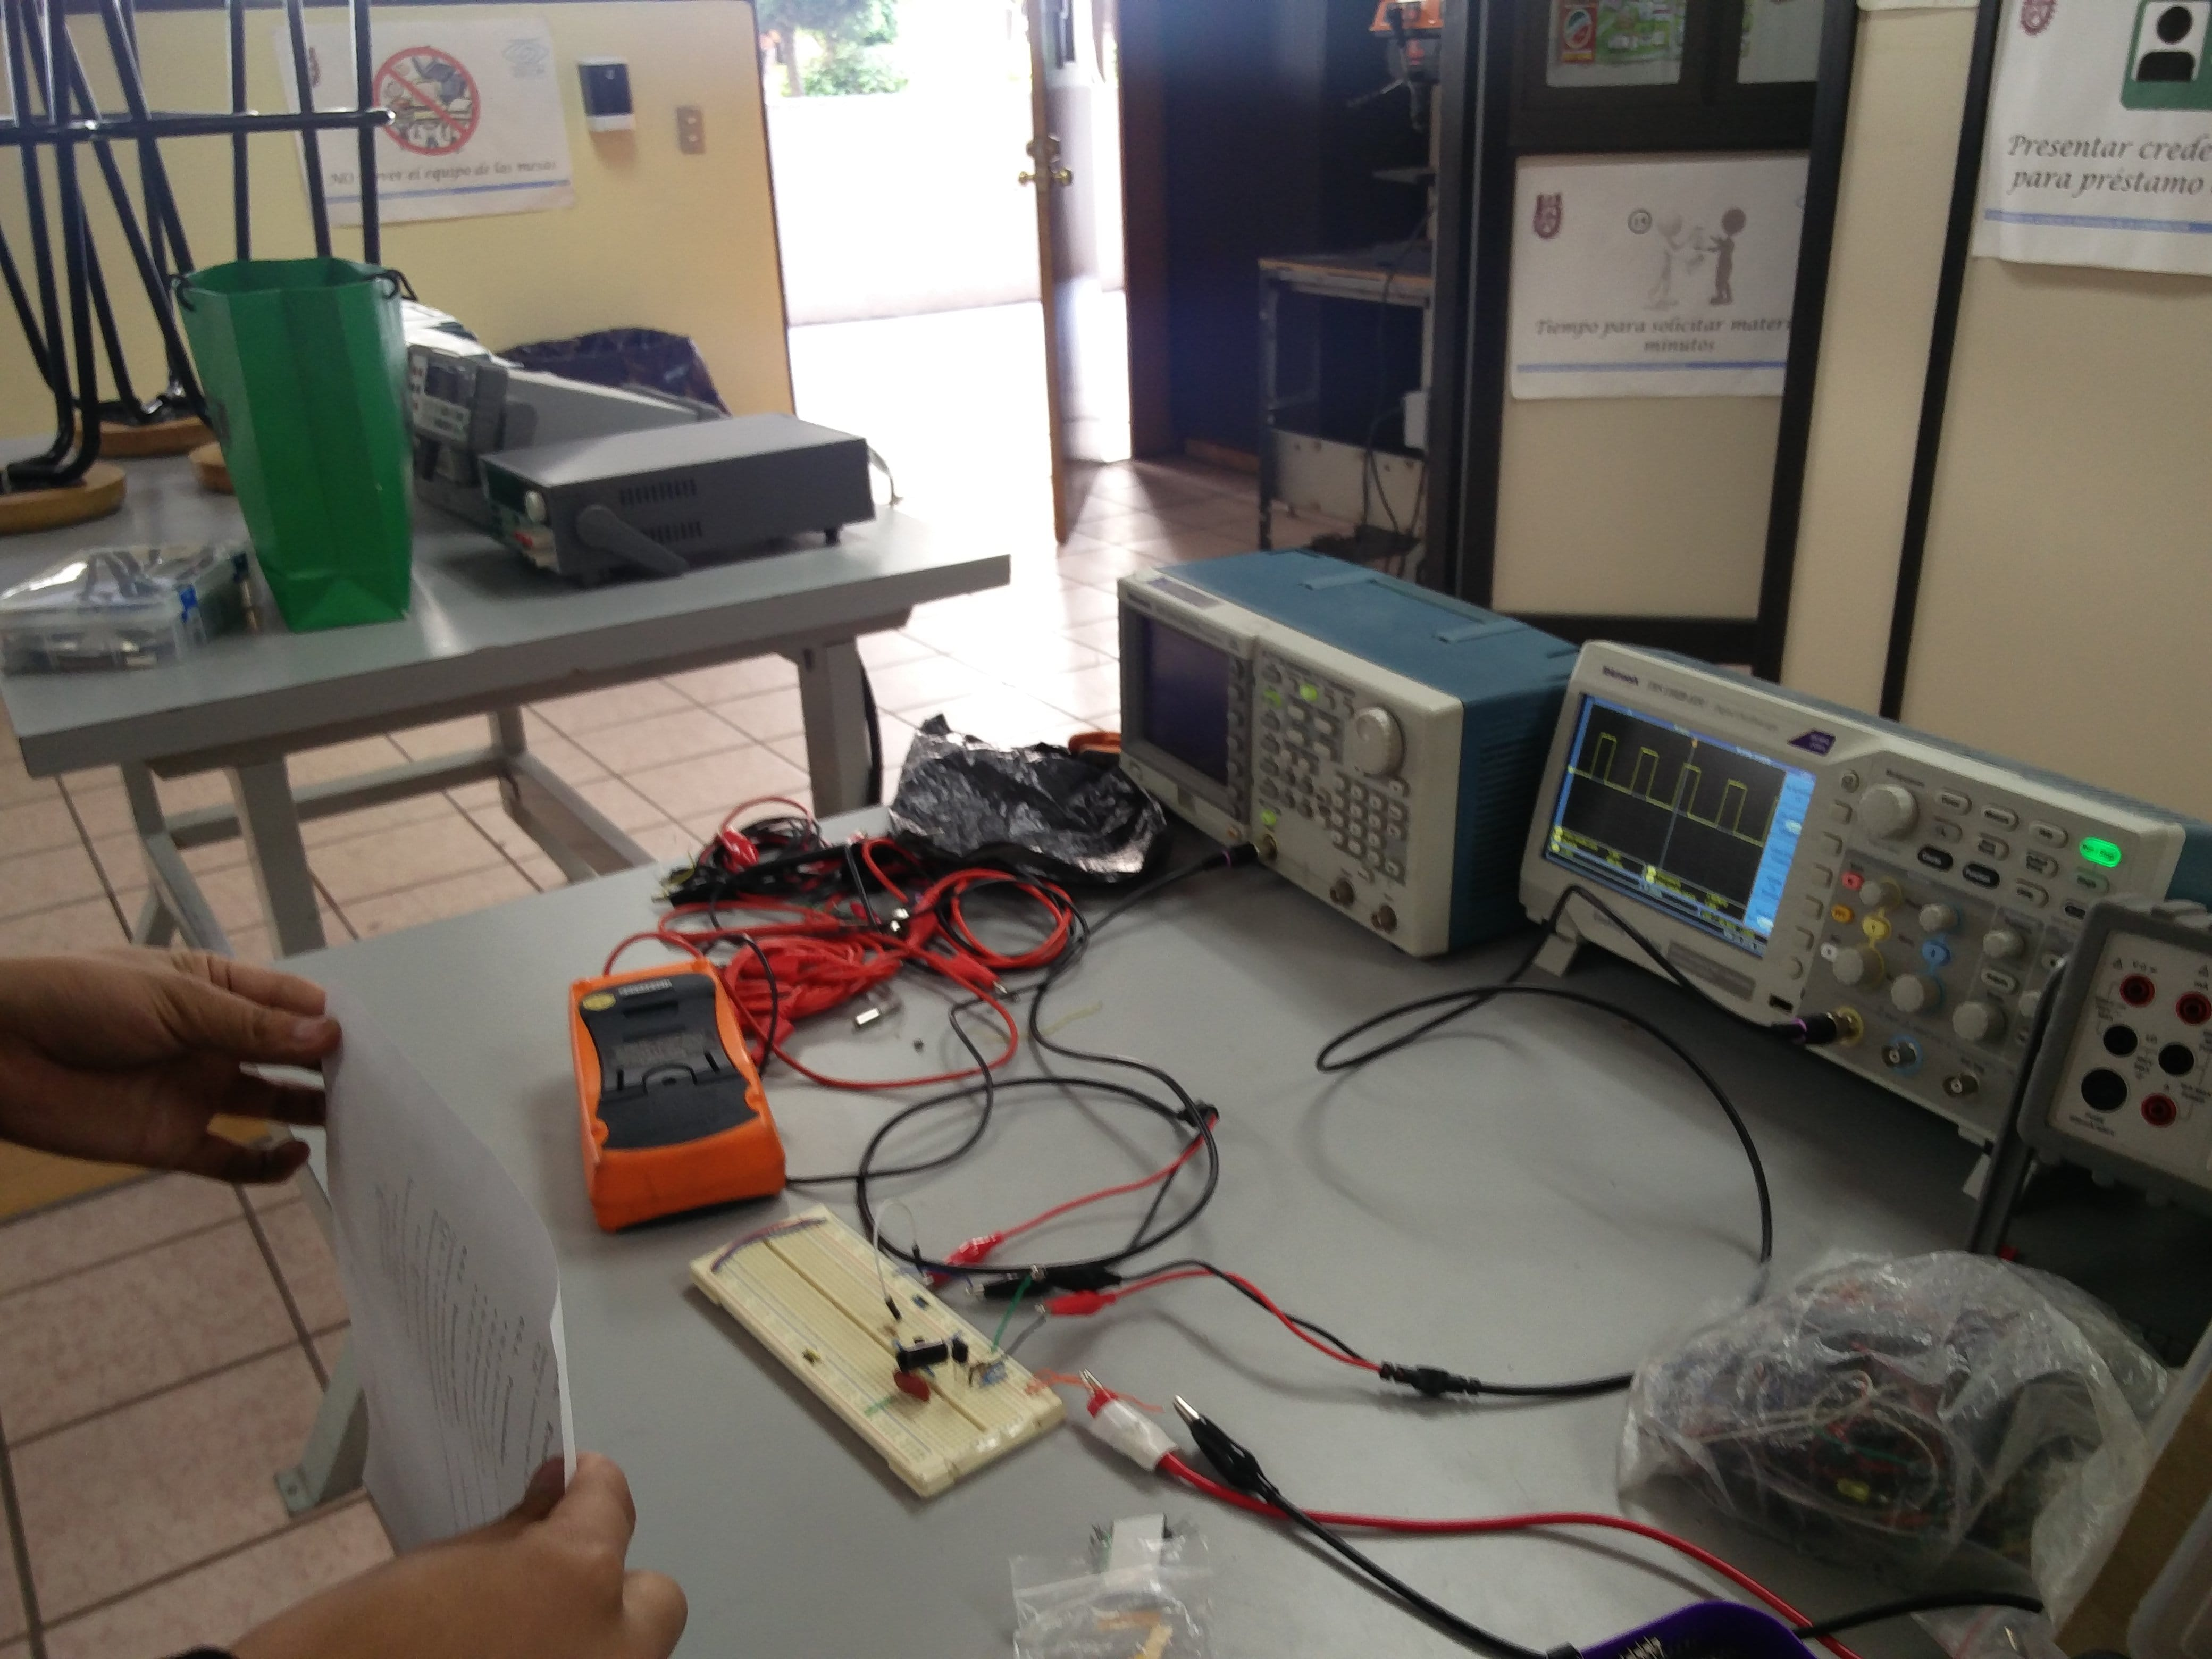
\includegraphics[width=0.4\textwidth]{5Distance}
            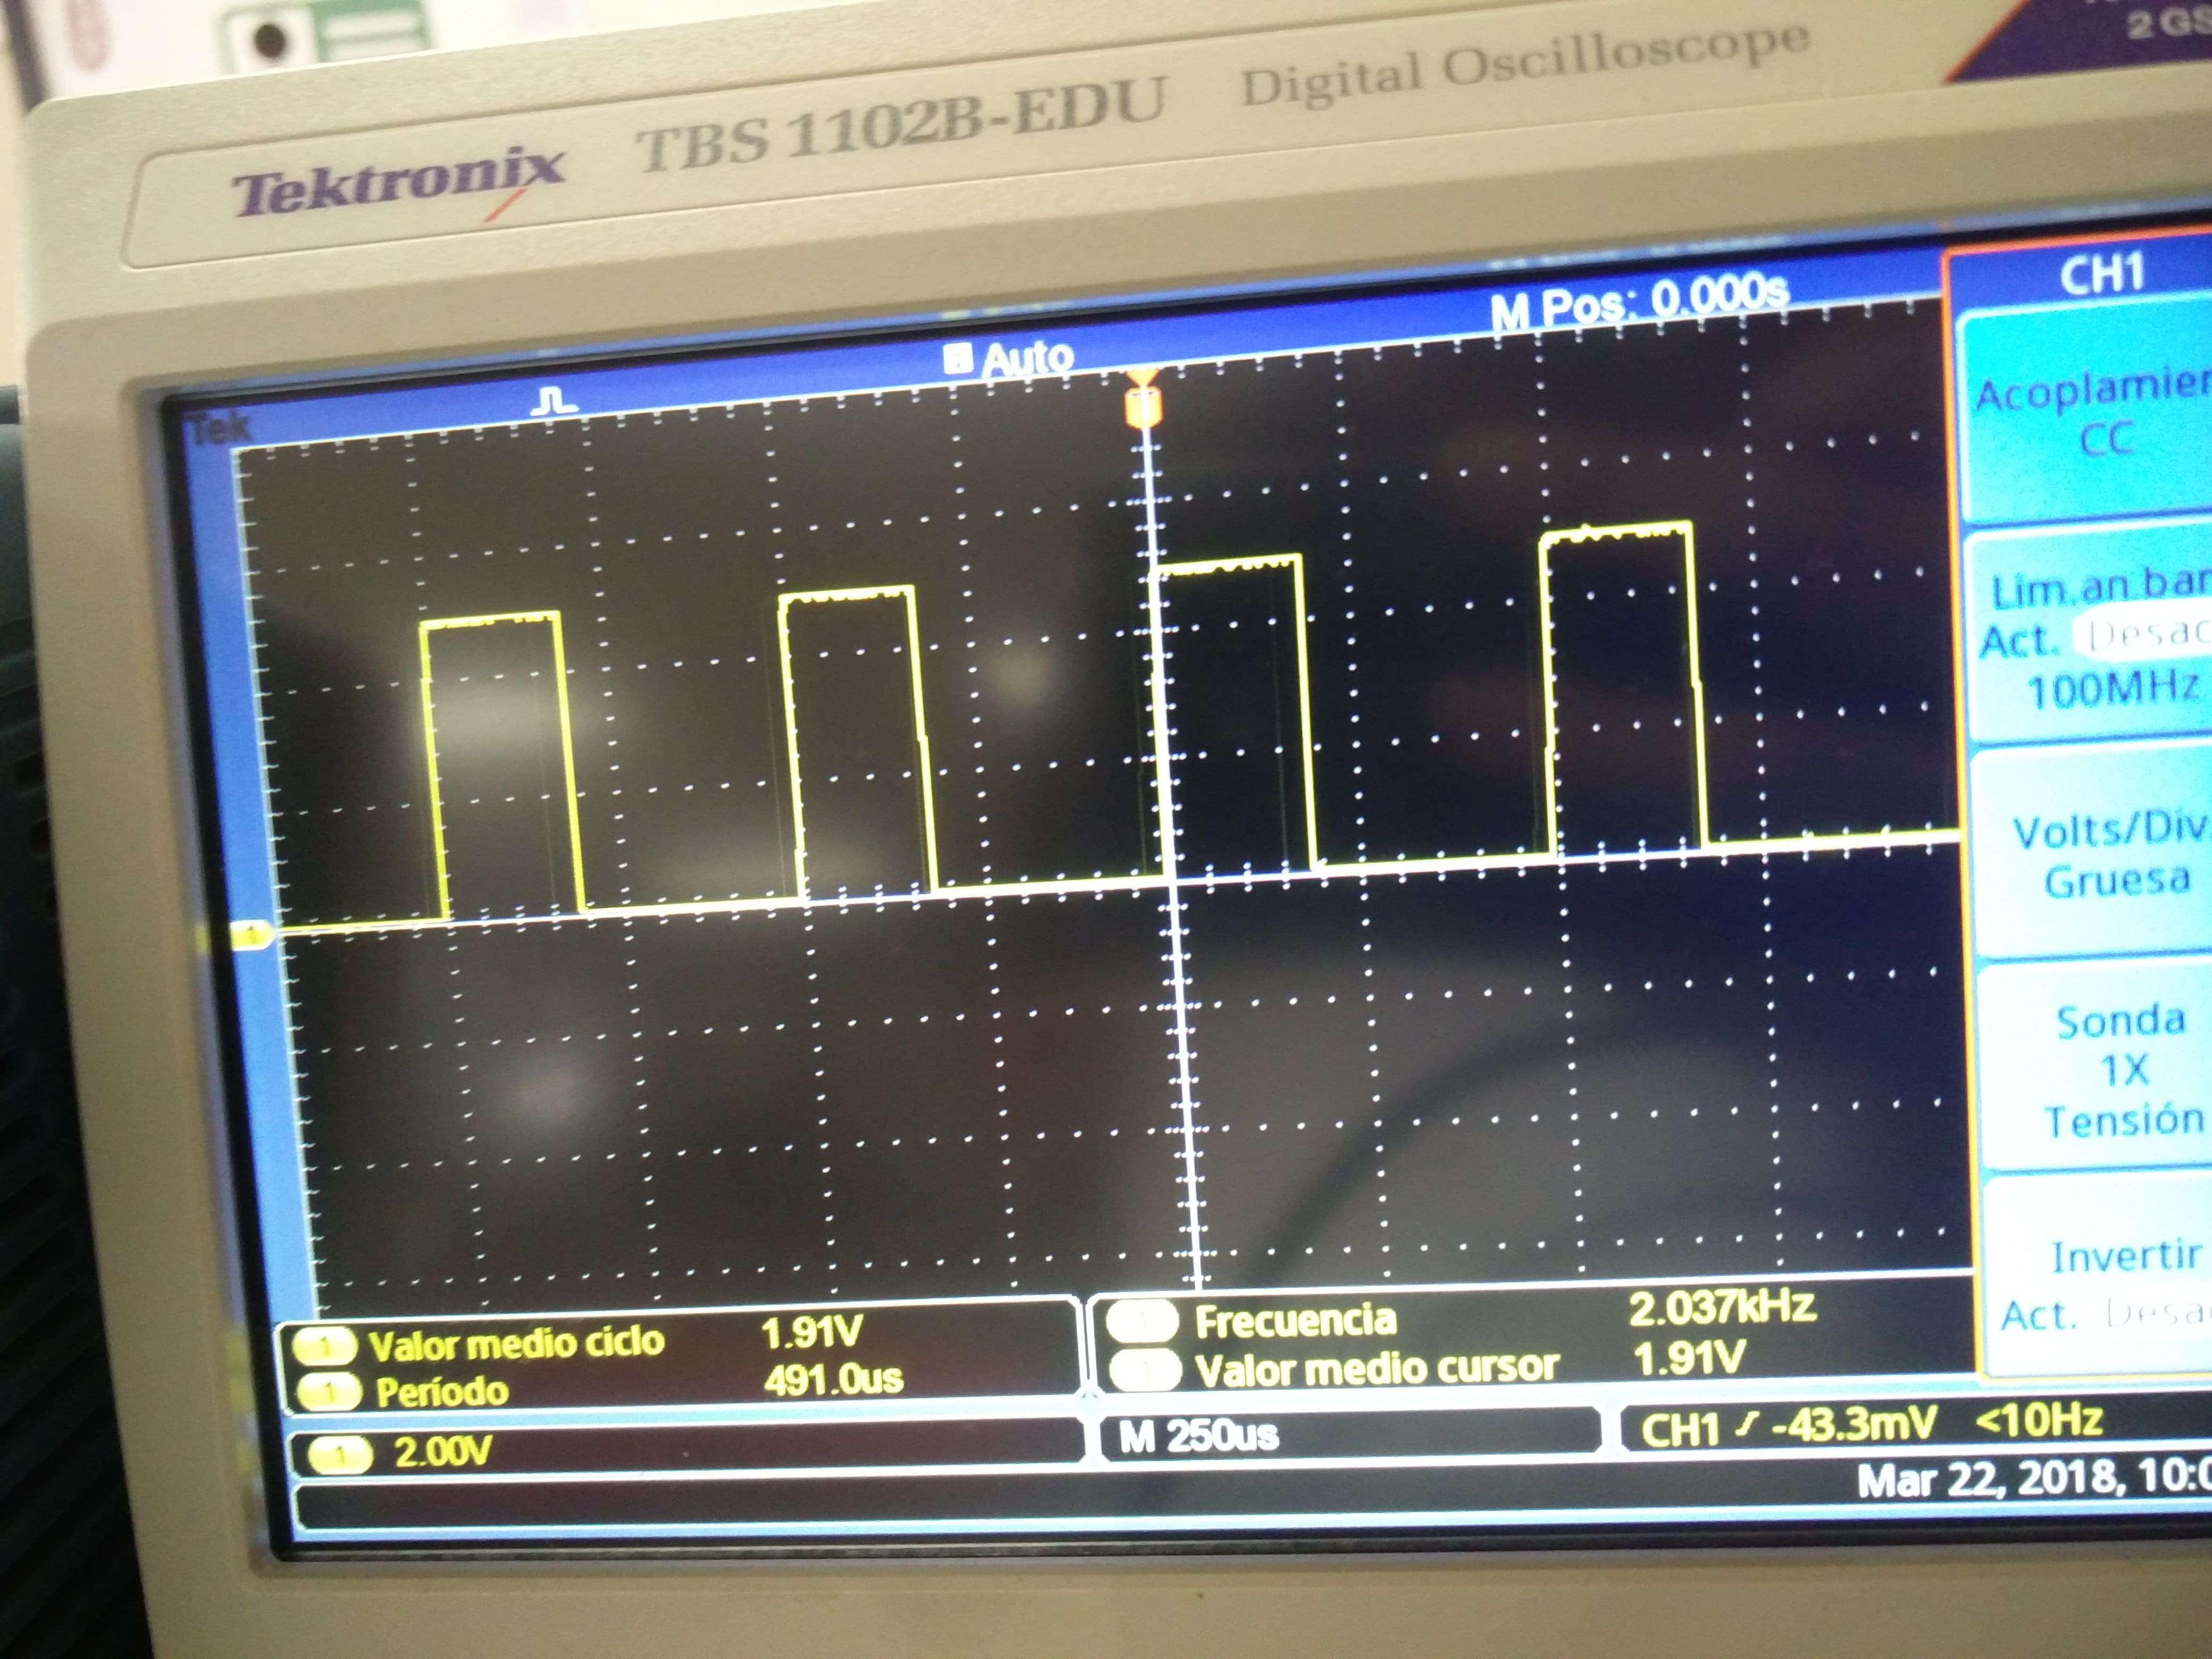
\includegraphics[width=0.4\textwidth]{5Signal}
        \end{figure}

        
        \clearpage

        $\sim$ 40 cm de Distancia
        \begin{figure}[h]
            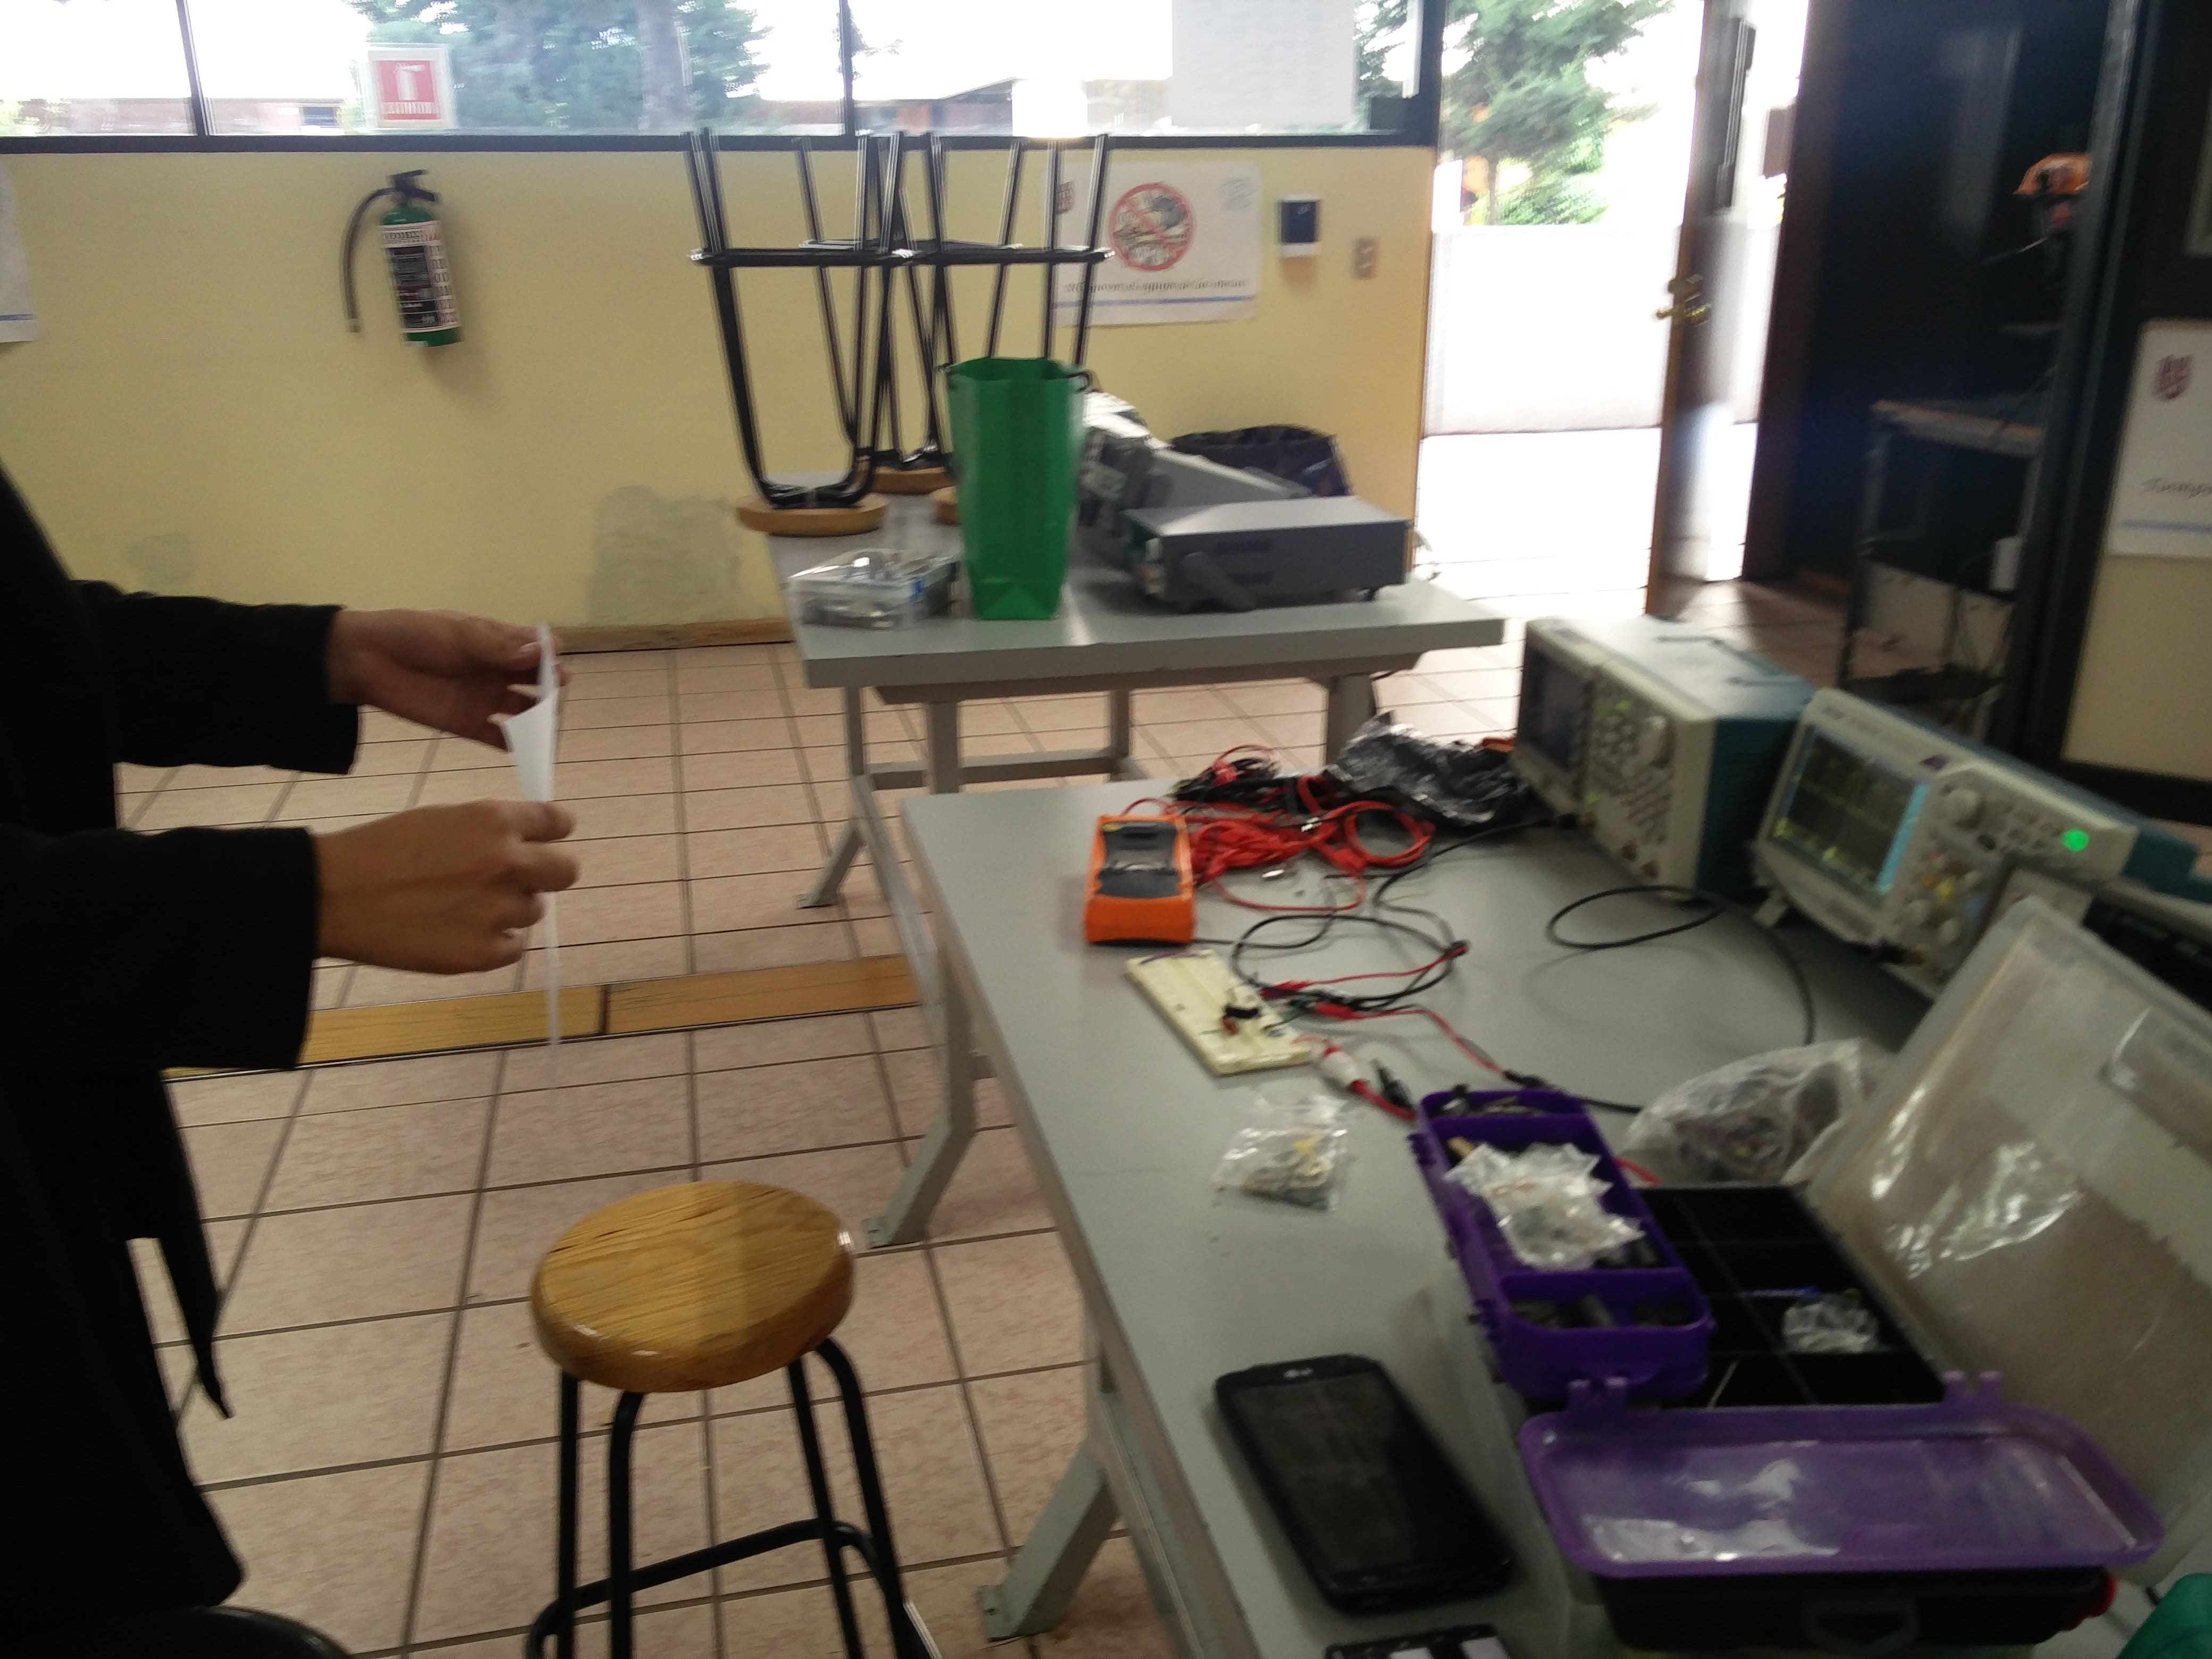
\includegraphics[width=0.4\textwidth]{6Distance}
            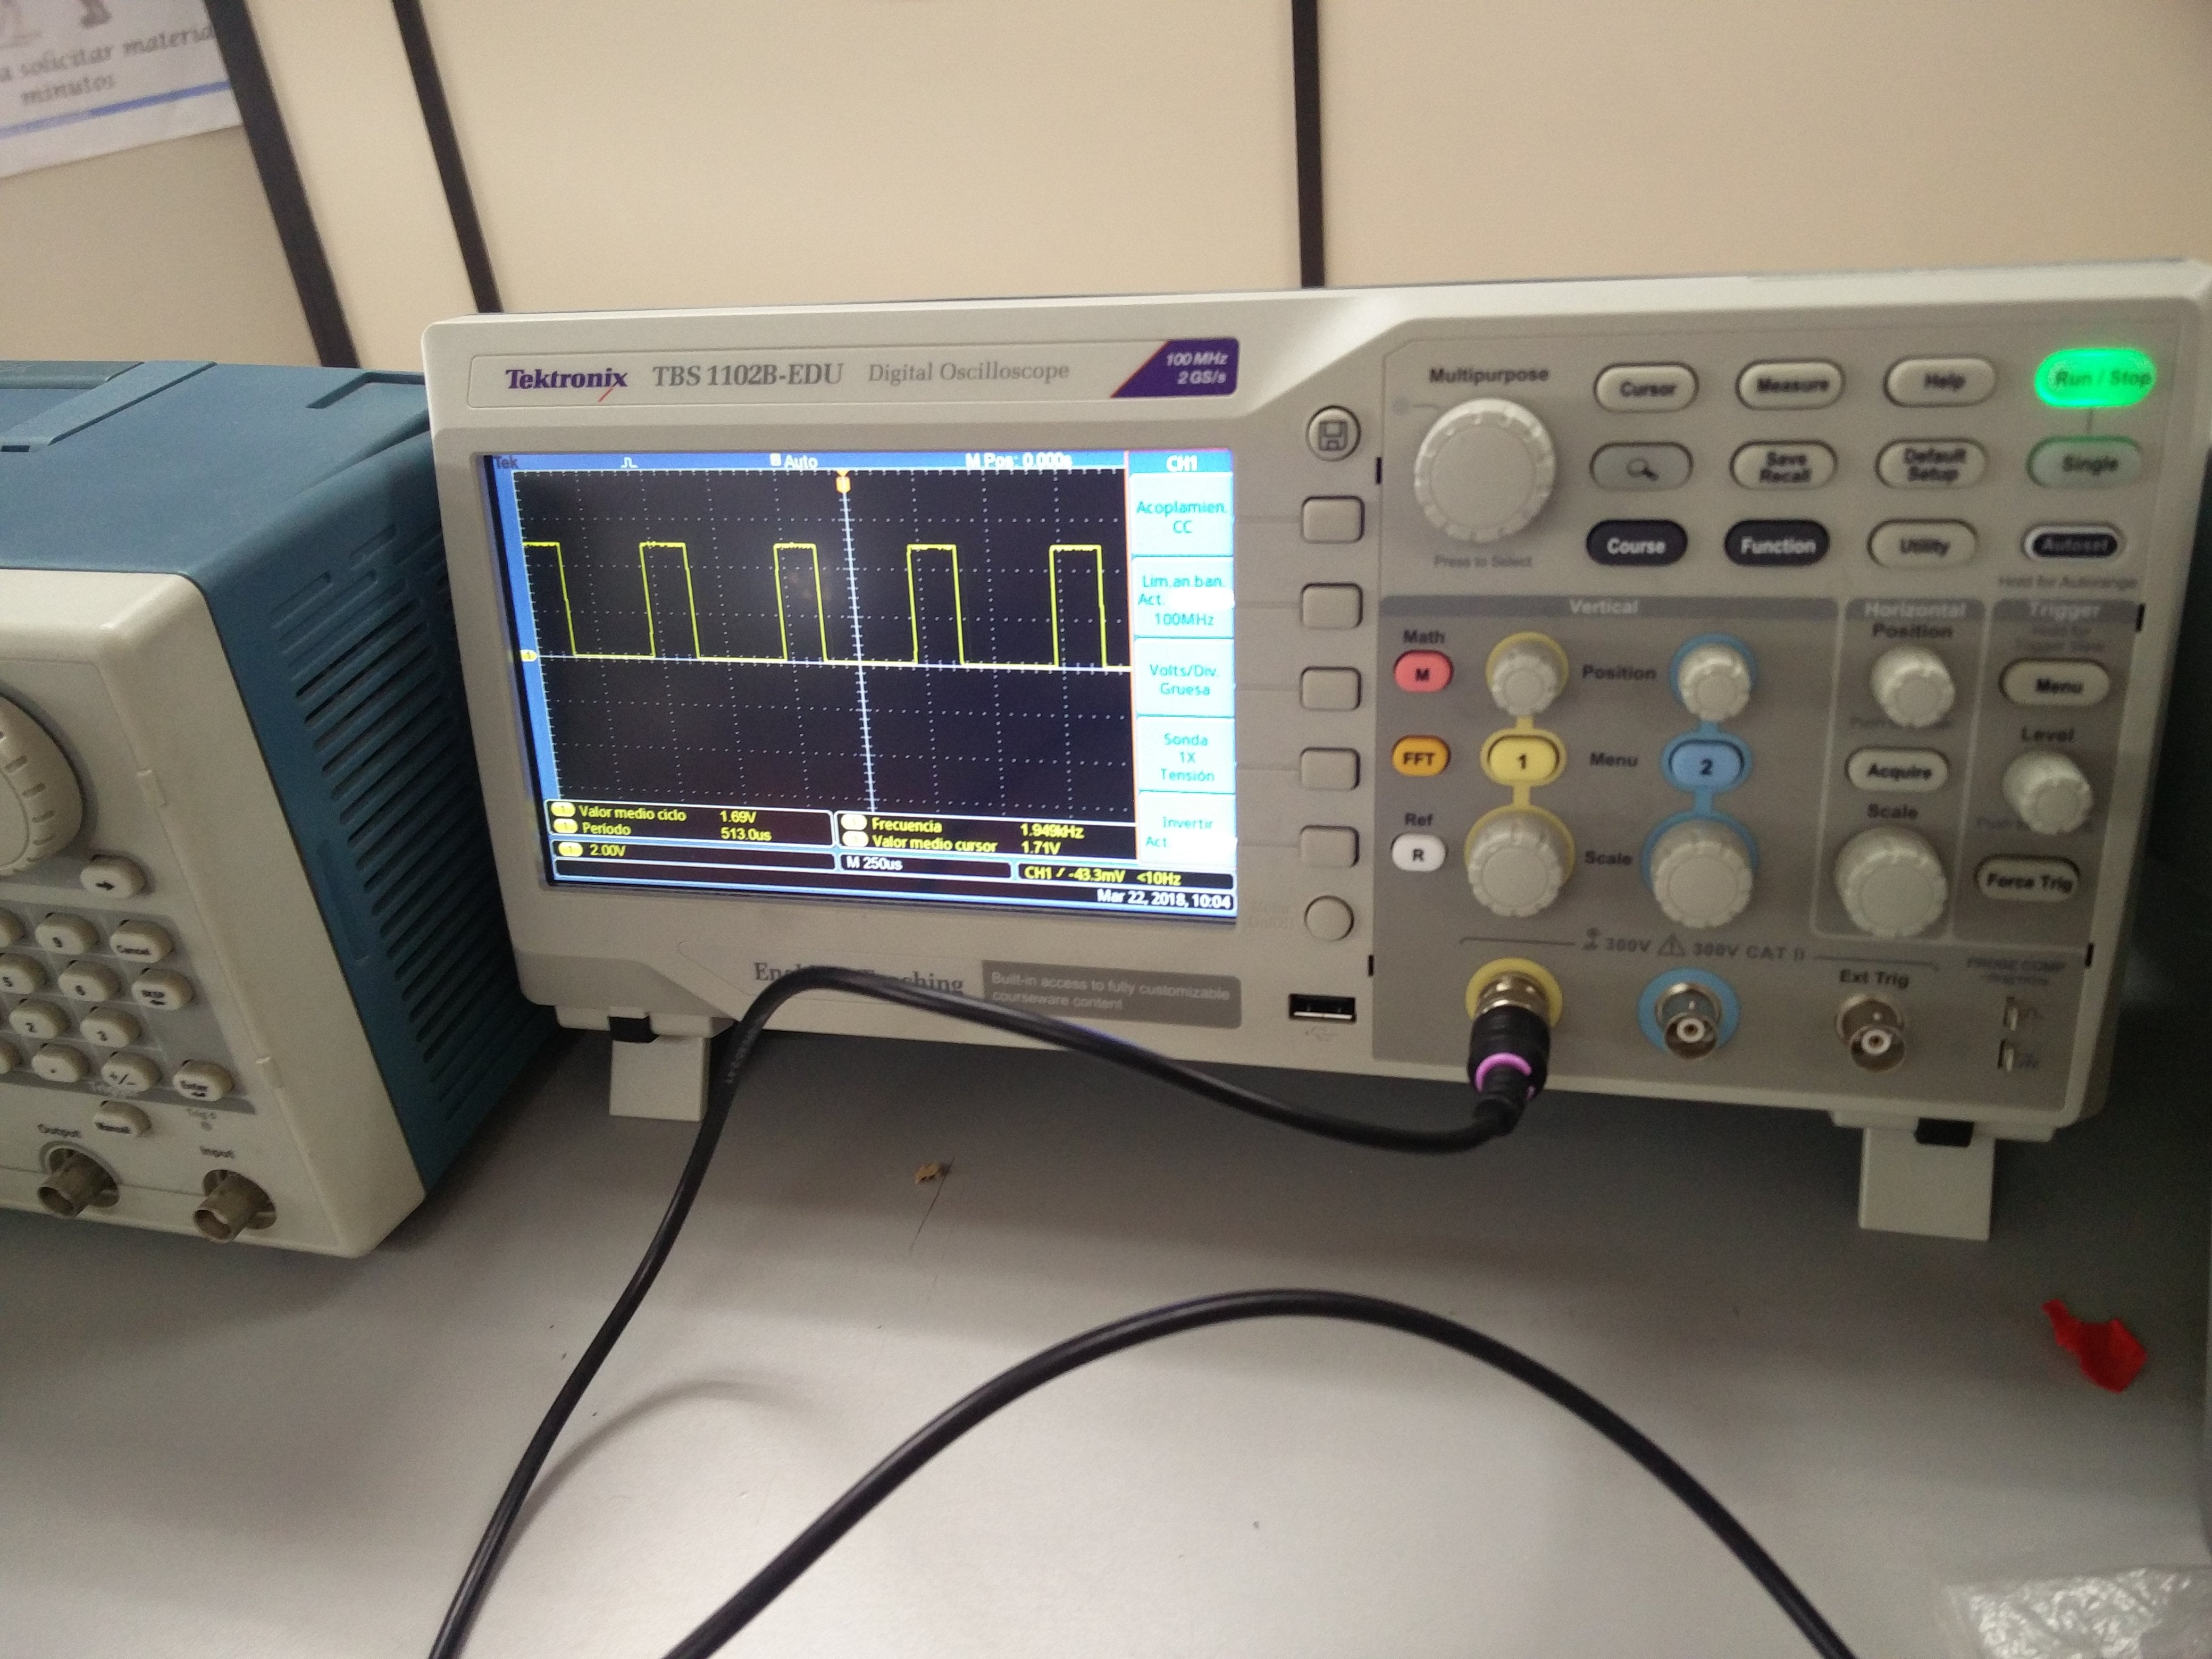
\includegraphics[width=0.4\textwidth]{6Signal}
        \end{figure}

        $\sim$ 70 cm de Distancia
        \begin{figure}[h]
            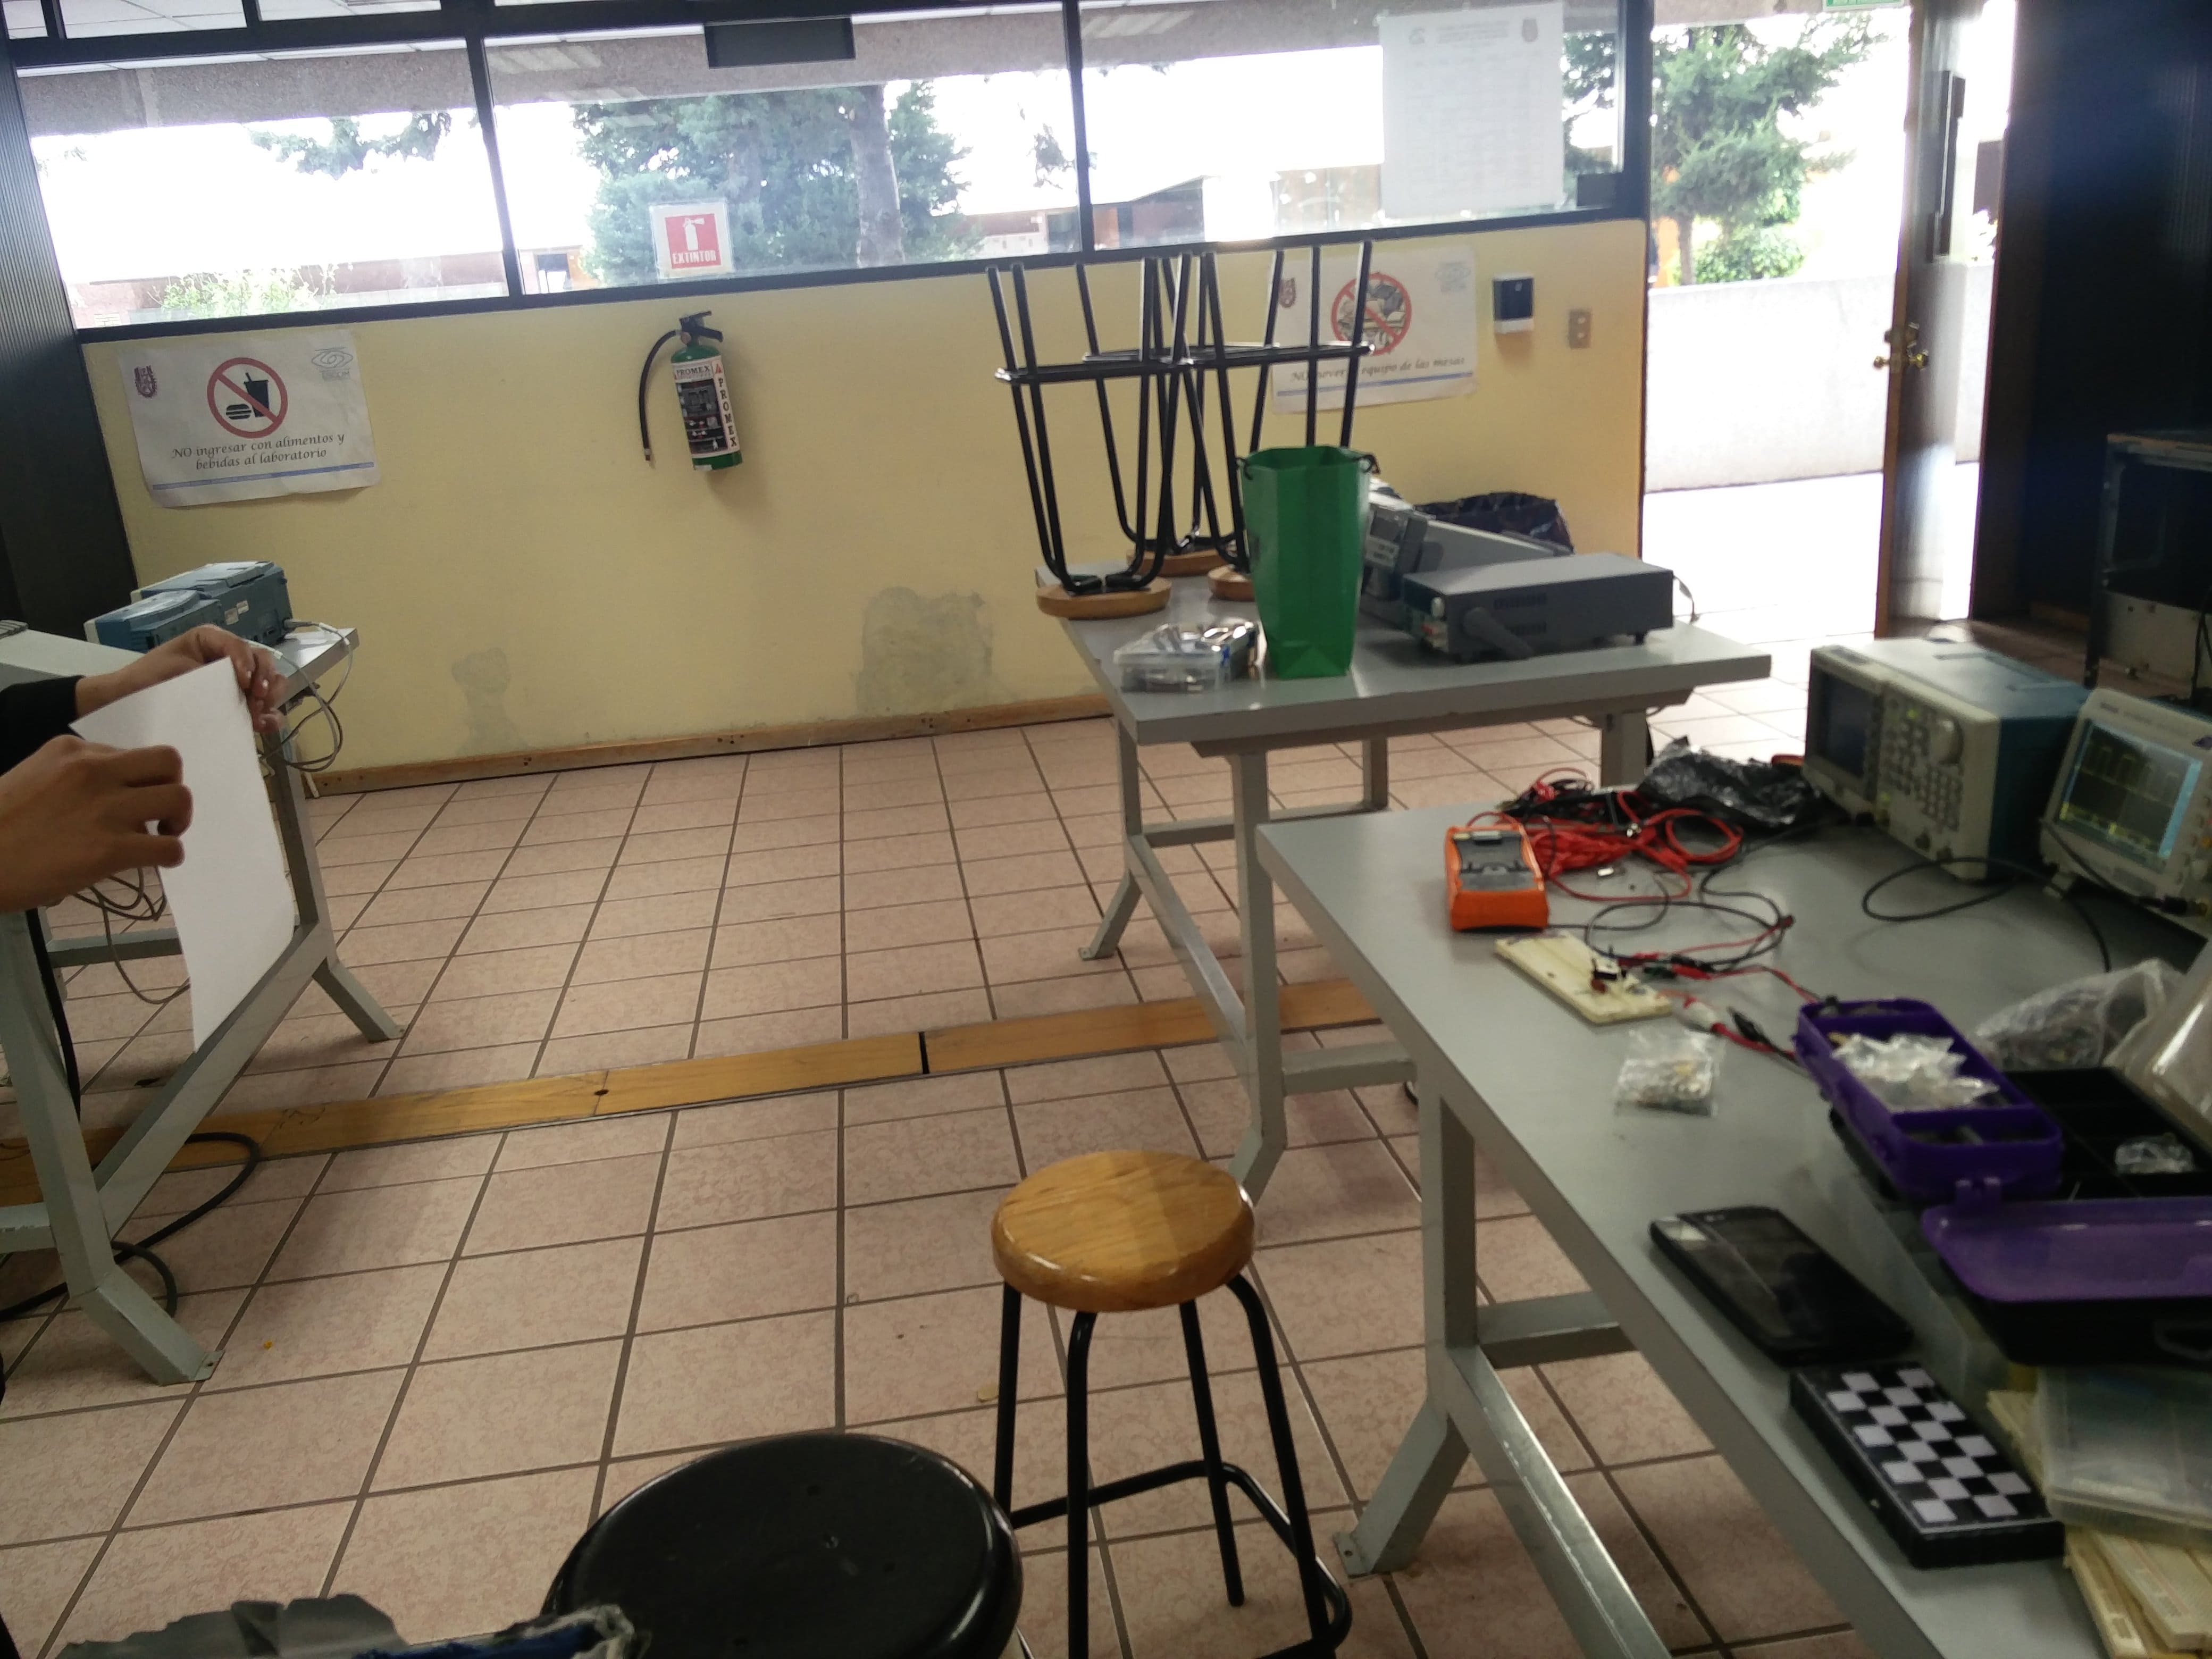
\includegraphics[width=0.4\textwidth]{2Distance}
            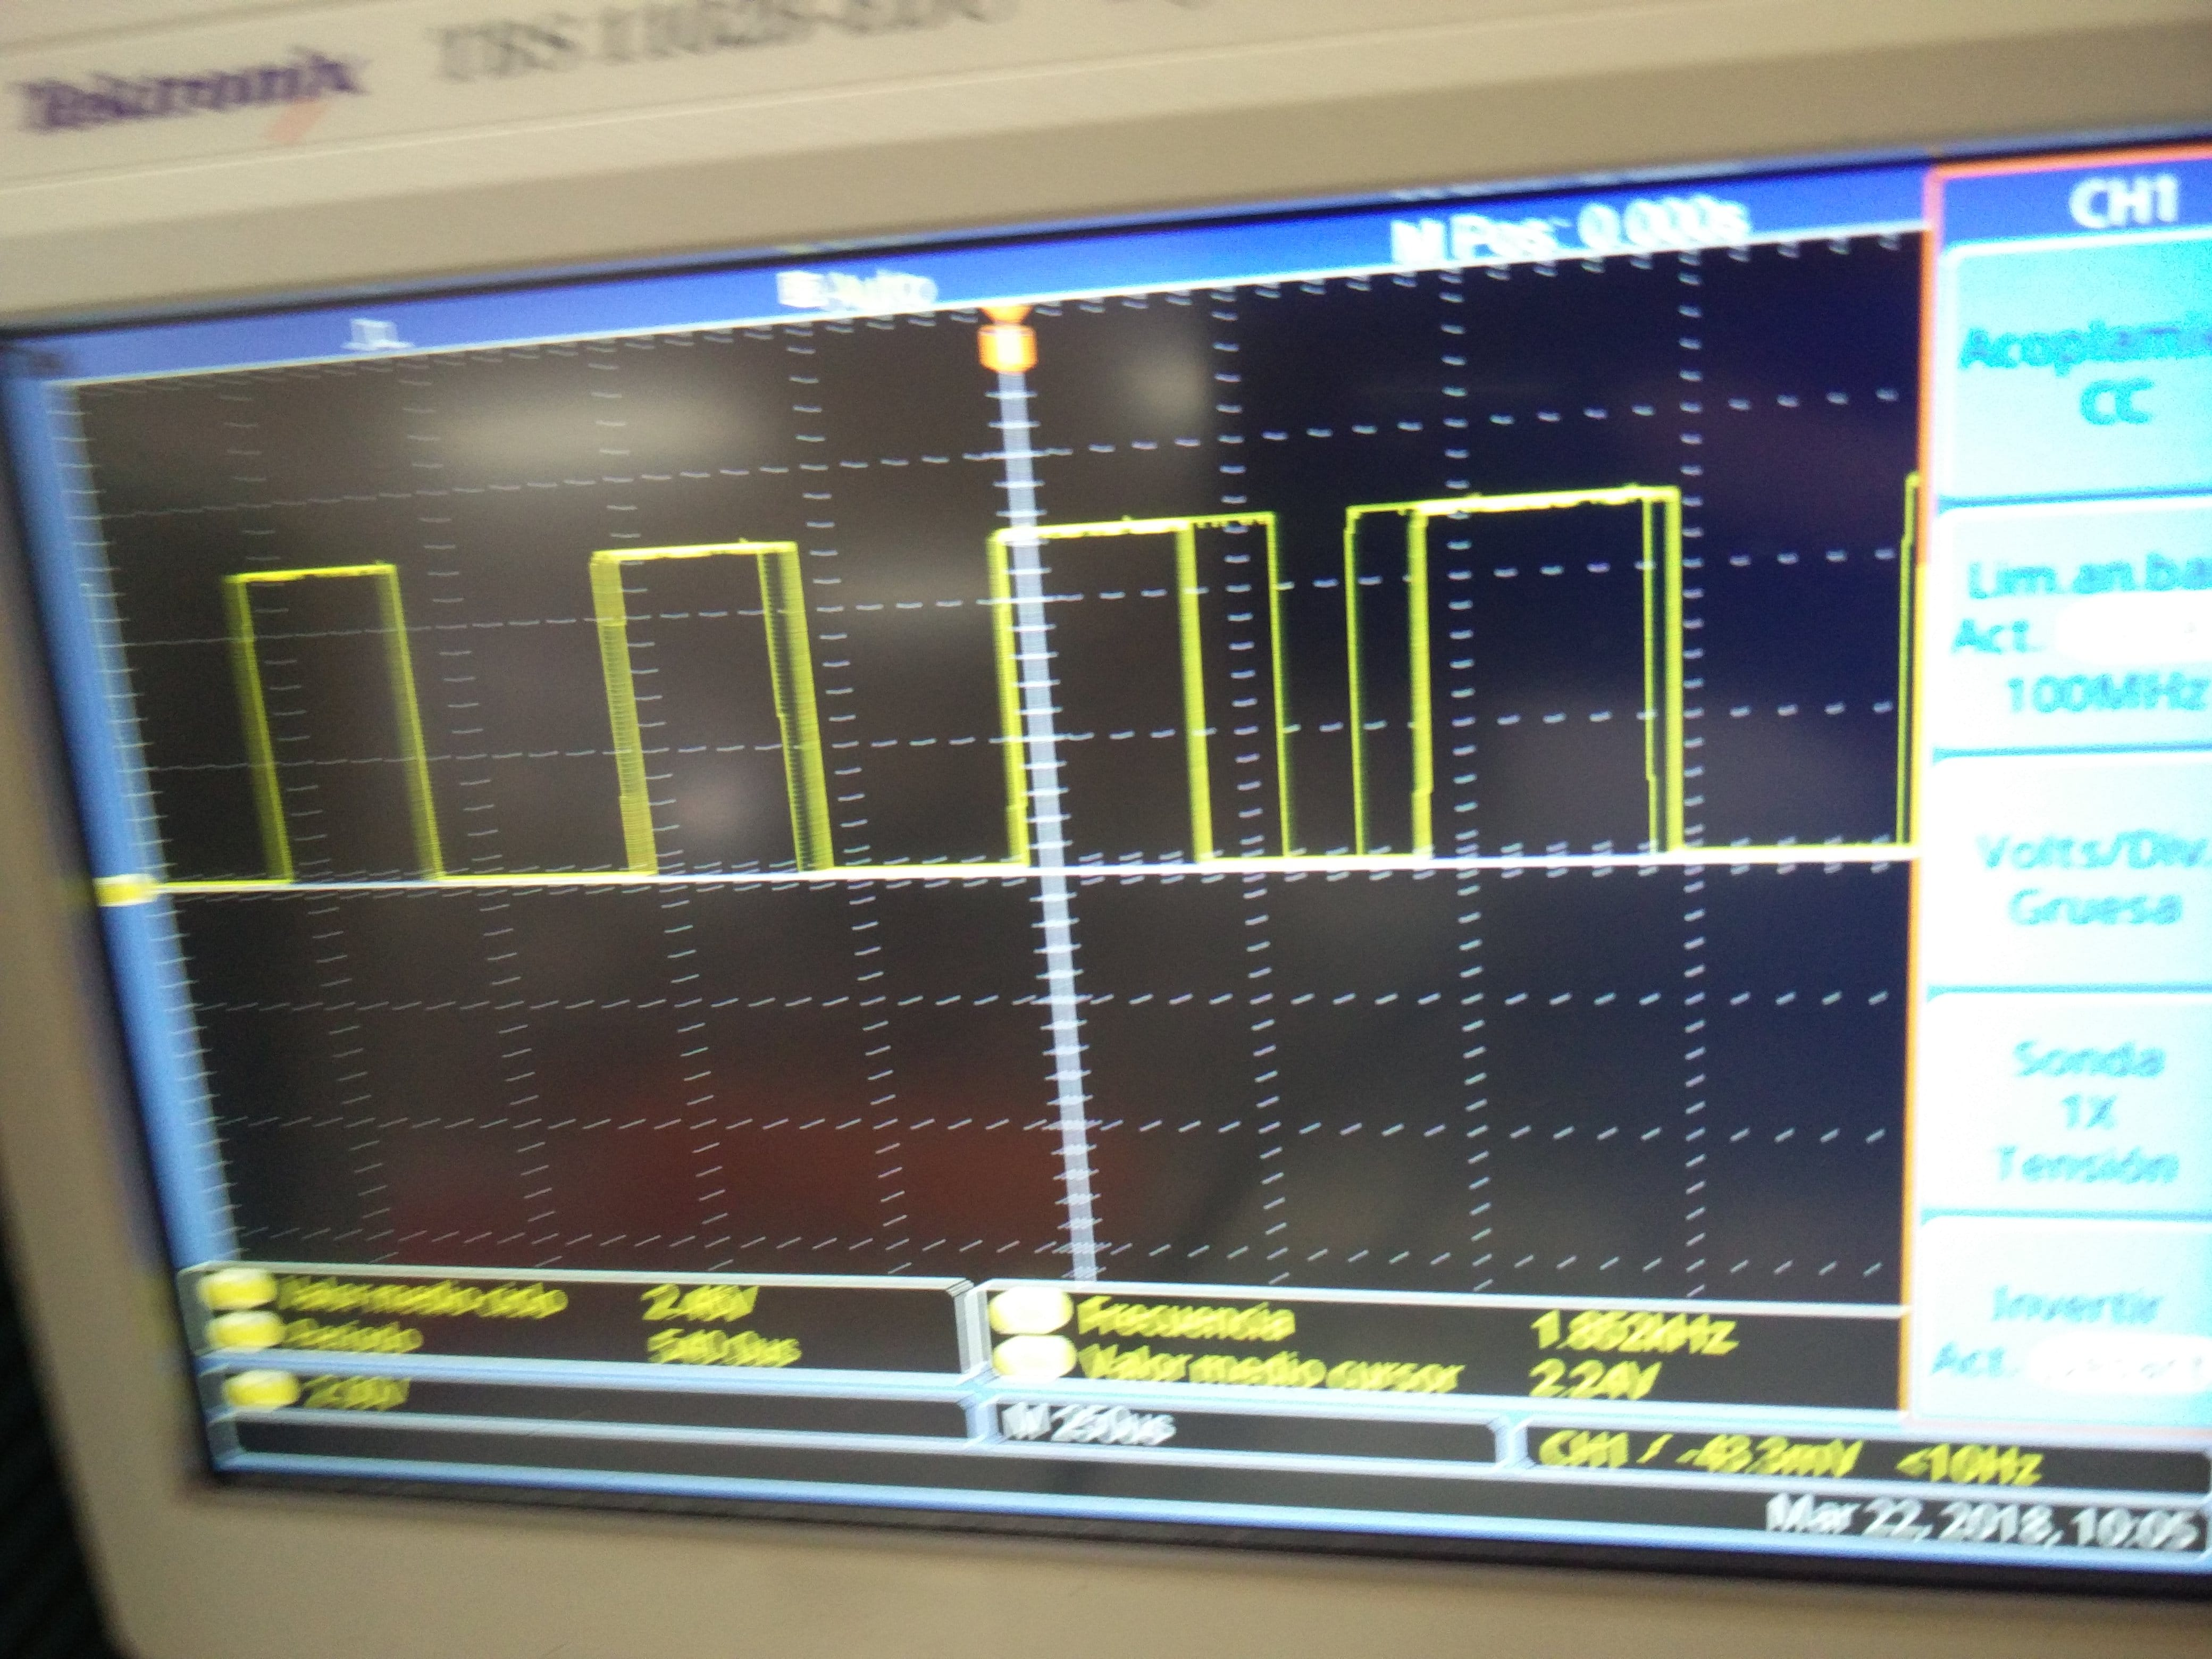
\includegraphics[width=0.4\textwidth]{2Signal}
        \end{figure}




    % ==============================================================
    % =============     CONCLUSIONES      ==========================
    % ==============================================================
    \clearpage
    \subsection{Conclusiones} 

        La práctica la logramos realizar con exito comprobando la funcionalidad del sensor
        para poder medir distancia de una manera relativamente precisa, así como vimos
        las diferencias en los sensores y la importancia de realizar los pulsos a determinadas
        frecuencias.

        Vimos como es que al conectarlo directamente a voltaje alcanzabamos un miserable rango de un par de
        centímetros, que se podían extender a casi un metro gracias a la modulación de pulsos cortos, esta
        fue la cable.

        Además que por la misma naturaleza, al enviar nuestra señal sobre una señal portadora, podiamos obtener
        nuestra señal de información sin problemas del otro lado, sin siquiera tener que eliminar le señal portadora.

        Eso si que fue una gran ventaja.

        Finalmente otro reto al que nos vimos envueltos es que el LED no disparaba su rayo unidireccionalmente
        sino que lo hacia de manera radial, por lo que incluso si la señal no rebotaba por triangulación, el receptor
        tenía la señal, por lo que tuvimos que usar un capuchon para hacer que la salida del LED fue unidireccional.

        Finalmente vimos que la calidad de la señal era gravemente adectada por los colores del objeto a medir, era muy
        difererente intentar medir una persona comparada con un caja negra, comparada con un papel blanco, esta es la
        principal razón por la cual nosotros no recomendaríamos usar este sensor como un sensor especializado a la hora de
        medir distancia.

        Eso, su limitado uso en exteriores y su dificultad para encontrar el angulo correcto a ciertas distancias.









\end{document}